\documentclass[twoside]{book}

% Packages required by doxygen
\usepackage{fixltx2e}
\usepackage{calc}
\usepackage{doxygen}
\usepackage[export]{adjustbox} % also loads graphicx
\usepackage{graphicx}
\usepackage[utf8]{inputenc}
\usepackage{makeidx}
\usepackage{multicol}
\usepackage{multirow}
\PassOptionsToPackage{warn}{textcomp}
\usepackage{textcomp}
\usepackage[nointegrals]{wasysym}
\usepackage[table]{xcolor}

% Font selection
\usepackage[T1]{fontenc}
\usepackage[scaled=.90]{helvet}
\usepackage{courier}
\usepackage{amssymb}
\usepackage{sectsty}
\renewcommand{\familydefault}{\sfdefault}
\allsectionsfont{%
  \fontseries{bc}\selectfont%
  \color{darkgray}%
}
\renewcommand{\DoxyLabelFont}{%
  \fontseries{bc}\selectfont%
  \color{darkgray}%
}
\newcommand{\+}{\discretionary{\mbox{\scriptsize$\hookleftarrow$}}{}{}}

% Page & text layout
\usepackage{geometry}
\geometry{%
  a4paper,%
  top=2.5cm,%
  bottom=2.5cm,%
  left=2.5cm,%
  right=2.5cm%
}
\tolerance=750
\hfuzz=15pt
\hbadness=750
\setlength{\emergencystretch}{15pt}
\setlength{\parindent}{0cm}
\setlength{\parskip}{3ex plus 2ex minus 2ex}
\makeatletter
\renewcommand{\paragraph}{%
  \@startsection{paragraph}{4}{0ex}{-1.0ex}{1.0ex}{%
    \normalfont\normalsize\bfseries\SS@parafont%
  }%
}
\renewcommand{\subparagraph}{%
  \@startsection{subparagraph}{5}{0ex}{-1.0ex}{1.0ex}{%
    \normalfont\normalsize\bfseries\SS@subparafont%
  }%
}
\makeatother

% Headers & footers
\usepackage{fancyhdr}
\pagestyle{fancyplain}
\fancyhead[LE]{\fancyplain{}{\bfseries\thepage}}
\fancyhead[CE]{\fancyplain{}{}}
\fancyhead[RE]{\fancyplain{}{\bfseries\leftmark}}
\fancyhead[LO]{\fancyplain{}{\bfseries\rightmark}}
\fancyhead[CO]{\fancyplain{}{}}
\fancyhead[RO]{\fancyplain{}{\bfseries\thepage}}
\fancyfoot[LE]{\fancyplain{}{}}
\fancyfoot[CE]{\fancyplain{}{}}
\fancyfoot[RE]{\fancyplain{}{\bfseries\scriptsize Generated by Doxygen }}
\fancyfoot[LO]{\fancyplain{}{\bfseries\scriptsize Generated by Doxygen }}
\fancyfoot[CO]{\fancyplain{}{}}
\fancyfoot[RO]{\fancyplain{}{}}
\renewcommand{\footrulewidth}{0.4pt}
\renewcommand{\chaptermark}[1]{%
  \markboth{#1}{}%
}
\renewcommand{\sectionmark}[1]{%
  \markright{\thesection\ #1}%
}

% Indices & bibliography
\usepackage{natbib}
\usepackage[titles]{tocloft}
\setcounter{tocdepth}{3}
\setcounter{secnumdepth}{5}
\makeindex

% Hyperlinks (required, but should be loaded last)
\usepackage{ifpdf}
\ifpdf
  \usepackage[pdftex,pagebackref=true]{hyperref}
\else
  \usepackage[ps2pdf,pagebackref=true]{hyperref}
\fi
\hypersetup{%
  colorlinks=true,%
  linkcolor=blue,%
  citecolor=blue,%
  unicode%
}

% Custom commands
\newcommand{\clearemptydoublepage}{%
  \newpage{\pagestyle{empty}\cleardoublepage}%
}

\usepackage{caption}
\captionsetup{labelsep=space,justification=centering,font={bf},singlelinecheck=off,skip=4pt,position=top}

%===== C O N T E N T S =====

\begin{document}

% Titlepage & ToC
\hypersetup{pageanchor=false,
             bookmarksnumbered=true,
             pdfencoding=unicode
            }
\pagenumbering{roman}
\begin{titlepage}
\vspace*{7cm}
\begin{center}%
{\Large My Project }\\
\vspace*{1cm}
{\large Generated by Doxygen 1.8.11}\\
\end{center}
\end{titlepage}
\clearemptydoublepage
\tableofcontents
\clearemptydoublepage
\pagenumbering{arabic}
\hypersetup{pageanchor=true}

%--- Begin generated contents ---
\chapter{R\+E\+A\+D\+ME}
\label{md_README}
\hypertarget{md_README}{}
Lendo bytecode de maneira legível para humanos\+: 
\begin{DoxyCode}
1 javap -v -p -s -sysinfo -constants ClaseExemplo.class
\end{DoxyCode}
 
\chapter{Class Index}
\section{Class List}
Here are the classes, structs, unions and interfaces with brief descriptions\+:\begin{DoxyCompactList}
\item\contentsline{section}{\hyperlink{structAppend__frame}{Append\+\_\+frame} }{\pageref{structAppend__frame}}{}
\item\contentsline{section}{\hyperlink{structattribute__info}{attribute\+\_\+info} }{\pageref{structattribute__info}}{}
\item\contentsline{section}{\hyperlink{unionattribute__types}{attribute\+\_\+types} }{\pageref{unionattribute__types}}{}
\item\contentsline{section}{\hyperlink{structBootstrap__method}{Bootstrap\+\_\+method} }{\pageref{structBootstrap__method}}{}
\item\contentsline{section}{\hyperlink{structChop__frame}{Chop\+\_\+frame} }{\pageref{structChop__frame}}{}
\item\contentsline{section}{\hyperlink{structClasses}{Classes} }{\pageref{structClasses}}{}
\item\contentsline{section}{\hyperlink{structClassFile}{Class\+File} }{\pageref{structClassFile}}{}
\item\contentsline{section}{\hyperlink{structcp__info}{cp\+\_\+info} }{\pageref{structcp__info}}{}
\item\contentsline{section}{\hyperlink{structDouble__variable__info}{Double\+\_\+variable\+\_\+info} }{\pageref{structDouble__variable__info}}{}
\item\contentsline{section}{\hyperlink{structexception__table__type}{exception\+\_\+table\+\_\+type} }{\pageref{structexception__table__type}}{}
\item\contentsline{section}{\hyperlink{structfield__info}{field\+\_\+info} }{\pageref{structfield__info}}{}
\item\contentsline{section}{\hyperlink{structFloat__variable__info}{Float\+\_\+variable\+\_\+info} }{\pageref{structFloat__variable__info}}{}
\item\contentsline{section}{\hyperlink{structFrame}{Frame} }{\pageref{structFrame}}{}
\item\contentsline{section}{\hyperlink{structFull__frame}{Full\+\_\+frame} }{\pageref{structFull__frame}}{}
\item\contentsline{section}{\hyperlink{structInteger__variable__info}{Integer\+\_\+variable\+\_\+info} }{\pageref{structInteger__variable__info}}{}
\item\contentsline{section}{\hyperlink{structJVM}{J\+VM} }{\pageref{structJVM}}{}
\item\contentsline{section}{\hyperlink{structline__number__table__type}{line\+\_\+number\+\_\+table\+\_\+type} }{\pageref{structline__number__table__type}}{}
\item\contentsline{section}{\hyperlink{structLocal__variable__table}{Local\+\_\+variable\+\_\+table} }{\pageref{structLocal__variable__table}}{}
\item\contentsline{section}{\hyperlink{structLocalVariable}{Local\+Variable} }{\pageref{structLocalVariable}}{}
\item\contentsline{section}{\hyperlink{structLong__variable__info}{Long\+\_\+variable\+\_\+info} }{\pageref{structLong__variable__info}}{}
\item\contentsline{section}{\hyperlink{structMethod}{Method} }{\pageref{structMethod}}{}
\item\contentsline{section}{\hyperlink{structmethod__info}{method\+\_\+info} }{\pageref{structmethod__info}}{}
\item\contentsline{section}{\hyperlink{structNull__variable__info}{Null\+\_\+variable\+\_\+info} }{\pageref{structNull__variable__info}}{}
\item\contentsline{section}{\hyperlink{structObject__variable__info}{Object\+\_\+variable\+\_\+info} }{\pageref{structObject__variable__info}}{}
\item\contentsline{section}{\hyperlink{structop__code}{op\+\_\+code} }{\pageref{structop__code}}{}
\item\contentsline{section}{\hyperlink{structSame__frame}{Same\+\_\+frame} }{\pageref{structSame__frame}}{}
\item\contentsline{section}{\hyperlink{structSame__frame__extended}{Same\+\_\+frame\+\_\+extended} }{\pageref{structSame__frame__extended}}{}
\item\contentsline{section}{\hyperlink{structSame__locals__1__stack__item__frame}{Same\+\_\+locals\+\_\+1\+\_\+stack\+\_\+item\+\_\+frame} }{\pageref{structSame__locals__1__stack__item__frame}}{}
\item\contentsline{section}{\hyperlink{structSame__locals__1__stack__item__frame__extended}{Same\+\_\+locals\+\_\+1\+\_\+stack\+\_\+item\+\_\+frame\+\_\+extended} }{\pageref{structSame__locals__1__stack__item__frame__extended}}{}
\item\contentsline{section}{\hyperlink{structstack__map__frame}{stack\+\_\+map\+\_\+frame} }{\pageref{structstack__map__frame}}{}
\item\contentsline{section}{\hyperlink{structStackFrame}{Stack\+Frame} }{\pageref{structStackFrame}}{}
\item\contentsline{section}{\hyperlink{structStackOperand}{Stack\+Operand} }{\pageref{structStackOperand}}{}
\item\contentsline{section}{\hyperlink{structTop__variable__info}{Top\+\_\+variable\+\_\+info} }{\pageref{structTop__variable__info}}{}
\item\contentsline{section}{\hyperlink{structTypeArray}{Type\+Array} }{\pageref{structTypeArray}}{}
\item\contentsline{section}{\hyperlink{structUninitialized__variable__info}{Uninitialized\+\_\+variable\+\_\+info} }{\pageref{structUninitialized__variable__info}}{}
\item\contentsline{section}{\hyperlink{structUninitializedThis__variable__info}{Uninitialized\+This\+\_\+variable\+\_\+info} }{\pageref{structUninitializedThis__variable__info}}{}
\item\contentsline{section}{\hyperlink{structverification__type__info}{verification\+\_\+type\+\_\+info} }{\pageref{structverification__type__info}}{}
\end{DoxyCompactList}

\chapter{Class Documentation}
\hypertarget{structAppend__frame}{}\section{Append\+\_\+frame Struct Reference}
\label{structAppend__frame}\index{Append\+\_\+frame@{Append\+\_\+frame}}


Collaboration diagram for Append\+\_\+frame\+:

\hypertarget{structattribute__info}{}\section{attribute\+\_\+info Struct Reference}
\label{structattribute__info}\index{attribute\+\_\+info@{attribute\+\_\+info}}


{\ttfamily \#include $<$structures.\+h$>$}



Collaboration diagram for attribute\+\_\+info\+:
% FIG 0
\subsection*{Public Attributes}
\begin{DoxyCompactItemize}
\item 
\hyperlink{structures_8h_a55ef8d87fd202b8417704c089899c5b9}{u2} \hyperlink{structattribute__info_a19df9d4b42eb55ca5dc1bed98df89378}{attribute\+\_\+name\+\_\+index}
\item 
\hyperlink{structures_8h_ae391a1d79bb0c8cbc283f0283e3c098b}{u4} \hyperlink{structattribute__info_a1ed8f679458c4bb0ed3315721588f50d}{attribute\+\_\+length}
\item 
\hyperlink{unionattribute__types}{attribute\+\_\+types} $\ast$ \hyperlink{structattribute__info_a78e740adccb41defb505248c47093958}{info}
\end{DoxyCompactItemize}


\subsection{Member Data Documentation}
\index{attribute\+\_\+info@{attribute\+\_\+info}!attribute\+\_\+length@{attribute\+\_\+length}}
\index{attribute\+\_\+length@{attribute\+\_\+length}!attribute\+\_\+info@{attribute\+\_\+info}}
\subsubsection[{\texorpdfstring{attribute\+\_\+length}{attribute_length}}]{\setlength{\rightskip}{0pt plus 5cm}{\bf u4} attribute\+\_\+info\+::attribute\+\_\+length}\hypertarget{structattribute__info_a1ed8f679458c4bb0ed3315721588f50d}{}\label{structattribute__info_a1ed8f679458c4bb0ed3315721588f50d}
\index{attribute\+\_\+info@{attribute\+\_\+info}!attribute\+\_\+name\+\_\+index@{attribute\+\_\+name\+\_\+index}}
\index{attribute\+\_\+name\+\_\+index@{attribute\+\_\+name\+\_\+index}!attribute\+\_\+info@{attribute\+\_\+info}}
\subsubsection[{\texorpdfstring{attribute\+\_\+name\+\_\+index}{attribute_name_index}}]{\setlength{\rightskip}{0pt plus 5cm}{\bf u2} attribute\+\_\+info\+::attribute\+\_\+name\+\_\+index}\hypertarget{structattribute__info_a19df9d4b42eb55ca5dc1bed98df89378}{}\label{structattribute__info_a19df9d4b42eb55ca5dc1bed98df89378}
\index{attribute\+\_\+info@{attribute\+\_\+info}!info@{info}}
\index{info@{info}!attribute\+\_\+info@{attribute\+\_\+info}}
\subsubsection[{\texorpdfstring{info}{info}}]{\setlength{\rightskip}{0pt plus 5cm}{\bf attribute\+\_\+types}$\ast$ attribute\+\_\+info\+::info}\hypertarget{structattribute__info_a78e740adccb41defb505248c47093958}{}\label{structattribute__info_a78e740adccb41defb505248c47093958}


The documentation for this struct was generated from the following file\+:\begin{DoxyCompactItemize}
\item 
\hyperlink{structures_8h}{structures.\+h}\end{DoxyCompactItemize}

\hypertarget{unionattribute__types}{}\section{attribute\+\_\+types Union Reference}
\label{unionattribute__types}\index{attribute\+\_\+types@{attribute\+\_\+types}}


Implementação dos atributos da \hyperlink{structJVM}{J\+VM} usando uma union.  




{\ttfamily \#include $<$structures.\+h$>$}



Collaboration diagram for attribute\+\_\+types\+:
% FIG 0
\subsection*{Public Attributes}
\begin{DoxyCompactItemize}
\item 
\begin{tabbing}
xx\=xx\=xx\=xx\=xx\=xx\=xx\=xx\=xx\=\kill
struct \{\\
\>\hyperlink{structures_8h_a55ef8d87fd202b8417704c089899c5b9}{u2} \hyperlink{unionattribute__types_abec9c5f39e4bfdc4de221e4645d15754}{constantvalue\_index}\\
\} \hyperlink{unionattribute__types_aaecd67000fbd2536ca5290a26b0413b0}{ConstantValue\_attribute}\\

\end{tabbing}\item 
\begin{tabbing}
xx\=xx\=xx\=xx\=xx\=xx\=xx\=xx\=xx\=\kill
struct \{\\
\>\hyperlink{structures_8h_a55ef8d87fd202b8417704c089899c5b9}{u2} \hyperlink{unionattribute__types_acef55ed8e6d377038f26e56398715ba3}{line\_number\_table\_length}\\
\>\hyperlink{structline__number__table__type}{line\_number\_table\_type} $\ast$ \hyperlink{unionattribute__types_af9c522c40e319223069c2aa95863aef1}{line\_number\_table}\\
\} \hyperlink{unionattribute__types_ac8d1e9ca062ca40620b53e65d67b78fd}{LineNumberTable\_attribute}\\

\end{tabbing}\item 
\begin{tabbing}
xx\=xx\=xx\=xx\=xx\=xx\=xx\=xx\=xx\=\kill
struct \{\\
\>\hyperlink{structures_8h_a55ef8d87fd202b8417704c089899c5b9}{u2} \hyperlink{unionattribute__types_a27a78095d45ab77a8670fe3d9c7fd349}{number\_of\_entries}\\
\>\hyperlink{structstack__map__frame}{stack\_map\_frame} $\ast$ \hyperlink{unionattribute__types_ac00cec5af4c5a187ddd975ce5cb2bc46}{entries}\\
\} \hyperlink{unionattribute__types_af40b8d96b4ed7c185e3bbe69ce26d920}{StackMapTable\_attribute}\\

\end{tabbing}\item 
\begin{tabbing}
xx\=xx\=xx\=xx\=xx\=xx\=xx\=xx\=xx\=\kill
struct \{\\
\>\hyperlink{structures_8h_a55ef8d87fd202b8417704c089899c5b9}{u2} \hyperlink{unionattribute__types_a28b4309a74ee5b3ea7d6738538c7a0d1}{sourcefile\_index}\\
\} \hyperlink{unionattribute__types_a4c070f5b3468652a8d4face97c3fc4e8}{SourceFile\_attribute}\\

\end{tabbing}\item 
\begin{tabbing}
xx\=xx\=xx\=xx\=xx\=xx\=xx\=xx\=xx\=\kill
struct \{\\
\} \hyperlink{unionattribute__types_a2c2fb712764e37c9caa0f7c9d83df51b}{Deprecated\_attribute}\\

\end{tabbing}\item 
\begin{tabbing}
xx\=xx\=xx\=xx\=xx\=xx\=xx\=xx\=xx\=\kill
struct \{\\
\>\hyperlink{structures_8h_a55ef8d87fd202b8417704c089899c5b9}{u2} \hyperlink{unionattribute__types_a748f9fb3ef2577233e061e356586bbbd}{number\_of\_exceptions}\\
\>\hyperlink{structures_8h_a55ef8d87fd202b8417704c089899c5b9}{u2} $\ast$ \hyperlink{unionattribute__types_a657fefd71fc9f8bd619852368844447e}{exception\_index\_table}\\
\} \hyperlink{unionattribute__types_ae3da53b0d811eb70361e1328db9b59e9}{Exceptions\_attribute}\\

\end{tabbing}\item 
\begin{tabbing}
xx\=xx\=xx\=xx\=xx\=xx\=xx\=xx\=xx\=\kill
struct \{\\
\>\hyperlink{structures_8h_a55ef8d87fd202b8417704c089899c5b9}{u2} \hyperlink{unionattribute__types_a70697a76d3152b6825b7a6e755cd7d52}{number\_of\_classes}\\
\>\hyperlink{structClasses}{Classes} $\ast$ \hyperlink{unionattribute__types_a8d9fb2d6b28b3da9923deae9e56cf807}{classes}\\
\} \hyperlink{unionattribute__types_af84c3875a56f217878eec232fe8e33f3}{InnerClasses\_attribute}\\

\end{tabbing}\item 
\begin{tabbing}
xx\=xx\=xx\=xx\=xx\=xx\=xx\=xx\=xx\=\kill
struct \{\\
\} \hyperlink{unionattribute__types_a04d1c36708ba372962219177169bedf1}{Synthetic\_attribute}\\

\end{tabbing}\item 
\begin{tabbing}
xx\=xx\=xx\=xx\=xx\=xx\=xx\=xx\=xx\=\kill
struct \{\\
\>\hyperlink{structures_8h_a55ef8d87fd202b8417704c089899c5b9}{u2} \hyperlink{unionattribute__types_ab1929338658430350fa68788fddd1441}{local\_variable\_table\_length}\\
\>\hyperlink{structLocal__variable__table}{Local\_variable\_table} $\ast$ \hyperlink{unionattribute__types_af1c6811b142b955d09aba9045832bbc4}{local\_variable\_table}\\
\} \hyperlink{unionattribute__types_a14bd080c2d4d5c855107ac67c2c3627c}{LocalVariableTable\_attribute}\\

\end{tabbing}\item 
\begin{tabbing}
xx\=xx\=xx\=xx\=xx\=xx\=xx\=xx\=xx\=\kill
struct \{\\
\>\hyperlink{structures_8h_a55ef8d87fd202b8417704c089899c5b9}{u2} \hyperlink{unionattribute__types_a6a050e29dab5344fc07b1303a928b838}{num\_bootstrap\_methods}\\
\>\hyperlink{structBootstrap__method}{Bootstrap\_method} $\ast$ \hyperlink{unionattribute__types_acd21ae085be3ee8608b86c367a5408be}{bootstrap\_methods}\\
\} \hyperlink{unionattribute__types_ab7d4f09668c4f457a4a5e76d31a961e5}{BootstrapMethods\_attribute}\\

\end{tabbing}\item 
\begin{tabbing}
xx\=xx\=xx\=xx\=xx\=xx\=xx\=xx\=xx\=\kill
struct \{\\
\>\hyperlink{structures_8h_a55ef8d87fd202b8417704c089899c5b9}{u2} \hyperlink{unionattribute__types_a8aef12d8fa3206bf9e5a4ffba0f27c43}{max\_stack}\\
\>\hyperlink{structures_8h_a55ef8d87fd202b8417704c089899c5b9}{u2} \hyperlink{unionattribute__types_a43257bb8c61a610246f334abc8776d3f}{max\_locals}\\
\>\hyperlink{structures_8h_ae391a1d79bb0c8cbc283f0283e3c098b}{u4} \hyperlink{unionattribute__types_a6b6b493d963093474ba6c55a19abb6e4}{code\_length}\\
\>\hyperlink{structures_8h_a64f8055b64cf2a4c299c841130c5c938}{u1} $\ast$ \hyperlink{unionattribute__types_a95ba29f957b7294764f797a396bed627}{code}\\
\>\hyperlink{structures_8h_a55ef8d87fd202b8417704c089899c5b9}{u2} \hyperlink{unionattribute__types_a057d74055d4fa64d0f5c93ede3b4e97f}{exception\_table\_length}\\
\>\hyperlink{structexception__table__type}{exception\_table\_type} $\ast$ \hyperlink{unionattribute__types_af61d8e6486ae314ba9bfc0f791bf7032}{exception\_table}\\
\>\hyperlink{structures_8h_a55ef8d87fd202b8417704c089899c5b9}{u2} \hyperlink{unionattribute__types_a9ef9c49c6e838abafc0e88a7969862a4}{attributes\_count}\\
\>\hyperlink{structattribute__info}{attribute\_info} $\ast$ \hyperlink{unionattribute__types_a1c56d2a7a4234ee27f831a0a81550ccb}{attributes}\\
\} \hyperlink{unionattribute__types_a4d78dcb1862f185b0d2eff1ce96aec71}{Code\_attribute}\\

\end{tabbing}\end{DoxyCompactItemize}


\subsection{Detailed Description}
Implementação dos atributos da \hyperlink{structJVM}{J\+VM} usando uma union. 

\subsection{Member Data Documentation}
\index{attribute\+\_\+types@{attribute\+\_\+types}!attributes@{attributes}}
\index{attributes@{attributes}!attribute\+\_\+types@{attribute\+\_\+types}}
\subsubsection[{\texorpdfstring{attributes}{attributes}}]{\setlength{\rightskip}{0pt plus 5cm}{\bf attribute\+\_\+info}$\ast$ attribute\+\_\+types\+::attributes}\hypertarget{unionattribute__types_a1c56d2a7a4234ee27f831a0a81550ccb}{}\label{unionattribute__types_a1c56d2a7a4234ee27f831a0a81550ccb}
\index{attribute\+\_\+types@{attribute\+\_\+types}!attributes\+\_\+count@{attributes\+\_\+count}}
\index{attributes\+\_\+count@{attributes\+\_\+count}!attribute\+\_\+types@{attribute\+\_\+types}}
\subsubsection[{\texorpdfstring{attributes\+\_\+count}{attributes_count}}]{\setlength{\rightskip}{0pt plus 5cm}{\bf u2} attribute\+\_\+types\+::attributes\+\_\+count}\hypertarget{unionattribute__types_a9ef9c49c6e838abafc0e88a7969862a4}{}\label{unionattribute__types_a9ef9c49c6e838abafc0e88a7969862a4}
\index{attribute\+\_\+types@{attribute\+\_\+types}!bootstrap\+\_\+methods@{bootstrap\+\_\+methods}}
\index{bootstrap\+\_\+methods@{bootstrap\+\_\+methods}!attribute\+\_\+types@{attribute\+\_\+types}}
\subsubsection[{\texorpdfstring{bootstrap\+\_\+methods}{bootstrap_methods}}]{\setlength{\rightskip}{0pt plus 5cm}{\bf Bootstrap\+\_\+method}$\ast$ attribute\+\_\+types\+::bootstrap\+\_\+methods}\hypertarget{unionattribute__types_acd21ae085be3ee8608b86c367a5408be}{}\label{unionattribute__types_acd21ae085be3ee8608b86c367a5408be}
\index{attribute\+\_\+types@{attribute\+\_\+types}!Bootstrap\+Methods\+\_\+attribute@{Bootstrap\+Methods\+\_\+attribute}}
\index{Bootstrap\+Methods\+\_\+attribute@{Bootstrap\+Methods\+\_\+attribute}!attribute\+\_\+types@{attribute\+\_\+types}}
\subsubsection[{\texorpdfstring{Bootstrap\+Methods\+\_\+attribute}{BootstrapMethods_attribute}}]{\setlength{\rightskip}{0pt plus 5cm}struct \{ ... \}   attribute\+\_\+types\+::\+Bootstrap\+Methods\+\_\+attribute}\hypertarget{unionattribute__types_ab7d4f09668c4f457a4a5e76d31a961e5}{}\label{unionattribute__types_ab7d4f09668c4f457a4a5e76d31a961e5}
\index{attribute\+\_\+types@{attribute\+\_\+types}!classes@{classes}}
\index{classes@{classes}!attribute\+\_\+types@{attribute\+\_\+types}}
\subsubsection[{\texorpdfstring{classes}{classes}}]{\setlength{\rightskip}{0pt plus 5cm}{\bf Classes}$\ast$ attribute\+\_\+types\+::classes}\hypertarget{unionattribute__types_a8d9fb2d6b28b3da9923deae9e56cf807}{}\label{unionattribute__types_a8d9fb2d6b28b3da9923deae9e56cf807}
\index{attribute\+\_\+types@{attribute\+\_\+types}!code@{code}}
\index{code@{code}!attribute\+\_\+types@{attribute\+\_\+types}}
\subsubsection[{\texorpdfstring{code}{code}}]{\setlength{\rightskip}{0pt plus 5cm}{\bf u1}$\ast$ attribute\+\_\+types\+::code}\hypertarget{unionattribute__types_a95ba29f957b7294764f797a396bed627}{}\label{unionattribute__types_a95ba29f957b7294764f797a396bed627}
\index{attribute\+\_\+types@{attribute\+\_\+types}!Code\+\_\+attribute@{Code\+\_\+attribute}}
\index{Code\+\_\+attribute@{Code\+\_\+attribute}!attribute\+\_\+types@{attribute\+\_\+types}}
\subsubsection[{\texorpdfstring{Code\+\_\+attribute}{Code_attribute}}]{\setlength{\rightskip}{0pt plus 5cm}struct \{ ... \}   attribute\+\_\+types\+::\+Code\+\_\+attribute}\hypertarget{unionattribute__types_a4d78dcb1862f185b0d2eff1ce96aec71}{}\label{unionattribute__types_a4d78dcb1862f185b0d2eff1ce96aec71}
\index{attribute\+\_\+types@{attribute\+\_\+types}!code\+\_\+length@{code\+\_\+length}}
\index{code\+\_\+length@{code\+\_\+length}!attribute\+\_\+types@{attribute\+\_\+types}}
\subsubsection[{\texorpdfstring{code\+\_\+length}{code_length}}]{\setlength{\rightskip}{0pt plus 5cm}{\bf u4} attribute\+\_\+types\+::code\+\_\+length}\hypertarget{unionattribute__types_a6b6b493d963093474ba6c55a19abb6e4}{}\label{unionattribute__types_a6b6b493d963093474ba6c55a19abb6e4}
\index{attribute\+\_\+types@{attribute\+\_\+types}!Constant\+Value\+\_\+attribute@{Constant\+Value\+\_\+attribute}}
\index{Constant\+Value\+\_\+attribute@{Constant\+Value\+\_\+attribute}!attribute\+\_\+types@{attribute\+\_\+types}}
\subsubsection[{\texorpdfstring{Constant\+Value\+\_\+attribute}{ConstantValue_attribute}}]{\setlength{\rightskip}{0pt plus 5cm}struct \{ ... \}   attribute\+\_\+types\+::\+Constant\+Value\+\_\+attribute}\hypertarget{unionattribute__types_aaecd67000fbd2536ca5290a26b0413b0}{}\label{unionattribute__types_aaecd67000fbd2536ca5290a26b0413b0}
\index{attribute\+\_\+types@{attribute\+\_\+types}!constantvalue\+\_\+index@{constantvalue\+\_\+index}}
\index{constantvalue\+\_\+index@{constantvalue\+\_\+index}!attribute\+\_\+types@{attribute\+\_\+types}}
\subsubsection[{\texorpdfstring{constantvalue\+\_\+index}{constantvalue_index}}]{\setlength{\rightskip}{0pt plus 5cm}{\bf u2} attribute\+\_\+types\+::constantvalue\+\_\+index}\hypertarget{unionattribute__types_abec9c5f39e4bfdc4de221e4645d15754}{}\label{unionattribute__types_abec9c5f39e4bfdc4de221e4645d15754}
\index{attribute\+\_\+types@{attribute\+\_\+types}!Deprecated\+\_\+attribute@{Deprecated\+\_\+attribute}}
\index{Deprecated\+\_\+attribute@{Deprecated\+\_\+attribute}!attribute\+\_\+types@{attribute\+\_\+types}}
\subsubsection[{\texorpdfstring{Deprecated\+\_\+attribute}{Deprecated_attribute}}]{\setlength{\rightskip}{0pt plus 5cm}struct \{ ... \}   attribute\+\_\+types\+::\+Deprecated\+\_\+attribute}\hypertarget{unionattribute__types_a2c2fb712764e37c9caa0f7c9d83df51b}{}\label{unionattribute__types_a2c2fb712764e37c9caa0f7c9d83df51b}
\index{attribute\+\_\+types@{attribute\+\_\+types}!entries@{entries}}
\index{entries@{entries}!attribute\+\_\+types@{attribute\+\_\+types}}
\subsubsection[{\texorpdfstring{entries}{entries}}]{\setlength{\rightskip}{0pt plus 5cm}{\bf stack\+\_\+map\+\_\+frame}$\ast$ attribute\+\_\+types\+::entries}\hypertarget{unionattribute__types_ac00cec5af4c5a187ddd975ce5cb2bc46}{}\label{unionattribute__types_ac00cec5af4c5a187ddd975ce5cb2bc46}
\index{attribute\+\_\+types@{attribute\+\_\+types}!exception\+\_\+index\+\_\+table@{exception\+\_\+index\+\_\+table}}
\index{exception\+\_\+index\+\_\+table@{exception\+\_\+index\+\_\+table}!attribute\+\_\+types@{attribute\+\_\+types}}
\subsubsection[{\texorpdfstring{exception\+\_\+index\+\_\+table}{exception_index_table}}]{\setlength{\rightskip}{0pt plus 5cm}{\bf u2}$\ast$ attribute\+\_\+types\+::exception\+\_\+index\+\_\+table}\hypertarget{unionattribute__types_a657fefd71fc9f8bd619852368844447e}{}\label{unionattribute__types_a657fefd71fc9f8bd619852368844447e}
\index{attribute\+\_\+types@{attribute\+\_\+types}!exception\+\_\+table@{exception\+\_\+table}}
\index{exception\+\_\+table@{exception\+\_\+table}!attribute\+\_\+types@{attribute\+\_\+types}}
\subsubsection[{\texorpdfstring{exception\+\_\+table}{exception_table}}]{\setlength{\rightskip}{0pt plus 5cm}{\bf exception\+\_\+table\+\_\+type}$\ast$ attribute\+\_\+types\+::exception\+\_\+table}\hypertarget{unionattribute__types_af61d8e6486ae314ba9bfc0f791bf7032}{}\label{unionattribute__types_af61d8e6486ae314ba9bfc0f791bf7032}
\index{attribute\+\_\+types@{attribute\+\_\+types}!exception\+\_\+table\+\_\+length@{exception\+\_\+table\+\_\+length}}
\index{exception\+\_\+table\+\_\+length@{exception\+\_\+table\+\_\+length}!attribute\+\_\+types@{attribute\+\_\+types}}
\subsubsection[{\texorpdfstring{exception\+\_\+table\+\_\+length}{exception_table_length}}]{\setlength{\rightskip}{0pt plus 5cm}{\bf u2} attribute\+\_\+types\+::exception\+\_\+table\+\_\+length}\hypertarget{unionattribute__types_a057d74055d4fa64d0f5c93ede3b4e97f}{}\label{unionattribute__types_a057d74055d4fa64d0f5c93ede3b4e97f}
\index{attribute\+\_\+types@{attribute\+\_\+types}!Exceptions\+\_\+attribute@{Exceptions\+\_\+attribute}}
\index{Exceptions\+\_\+attribute@{Exceptions\+\_\+attribute}!attribute\+\_\+types@{attribute\+\_\+types}}
\subsubsection[{\texorpdfstring{Exceptions\+\_\+attribute}{Exceptions_attribute}}]{\setlength{\rightskip}{0pt plus 5cm}struct \{ ... \}   attribute\+\_\+types\+::\+Exceptions\+\_\+attribute}\hypertarget{unionattribute__types_ae3da53b0d811eb70361e1328db9b59e9}{}\label{unionattribute__types_ae3da53b0d811eb70361e1328db9b59e9}
\index{attribute\+\_\+types@{attribute\+\_\+types}!Inner\+Classes\+\_\+attribute@{Inner\+Classes\+\_\+attribute}}
\index{Inner\+Classes\+\_\+attribute@{Inner\+Classes\+\_\+attribute}!attribute\+\_\+types@{attribute\+\_\+types}}
\subsubsection[{\texorpdfstring{Inner\+Classes\+\_\+attribute}{InnerClasses_attribute}}]{\setlength{\rightskip}{0pt plus 5cm}struct \{ ... \}   attribute\+\_\+types\+::\+Inner\+Classes\+\_\+attribute}\hypertarget{unionattribute__types_af84c3875a56f217878eec232fe8e33f3}{}\label{unionattribute__types_af84c3875a56f217878eec232fe8e33f3}
\index{attribute\+\_\+types@{attribute\+\_\+types}!line\+\_\+number\+\_\+table@{line\+\_\+number\+\_\+table}}
\index{line\+\_\+number\+\_\+table@{line\+\_\+number\+\_\+table}!attribute\+\_\+types@{attribute\+\_\+types}}
\subsubsection[{\texorpdfstring{line\+\_\+number\+\_\+table}{line_number_table}}]{\setlength{\rightskip}{0pt plus 5cm}{\bf line\+\_\+number\+\_\+table\+\_\+type}$\ast$ attribute\+\_\+types\+::line\+\_\+number\+\_\+table}\hypertarget{unionattribute__types_af9c522c40e319223069c2aa95863aef1}{}\label{unionattribute__types_af9c522c40e319223069c2aa95863aef1}
\index{attribute\+\_\+types@{attribute\+\_\+types}!line\+\_\+number\+\_\+table\+\_\+length@{line\+\_\+number\+\_\+table\+\_\+length}}
\index{line\+\_\+number\+\_\+table\+\_\+length@{line\+\_\+number\+\_\+table\+\_\+length}!attribute\+\_\+types@{attribute\+\_\+types}}
\subsubsection[{\texorpdfstring{line\+\_\+number\+\_\+table\+\_\+length}{line_number_table_length}}]{\setlength{\rightskip}{0pt plus 5cm}{\bf u2} attribute\+\_\+types\+::line\+\_\+number\+\_\+table\+\_\+length}\hypertarget{unionattribute__types_acef55ed8e6d377038f26e56398715ba3}{}\label{unionattribute__types_acef55ed8e6d377038f26e56398715ba3}
\index{attribute\+\_\+types@{attribute\+\_\+types}!Line\+Number\+Table\+\_\+attribute@{Line\+Number\+Table\+\_\+attribute}}
\index{Line\+Number\+Table\+\_\+attribute@{Line\+Number\+Table\+\_\+attribute}!attribute\+\_\+types@{attribute\+\_\+types}}
\subsubsection[{\texorpdfstring{Line\+Number\+Table\+\_\+attribute}{LineNumberTable_attribute}}]{\setlength{\rightskip}{0pt plus 5cm}struct \{ ... \}   attribute\+\_\+types\+::\+Line\+Number\+Table\+\_\+attribute}\hypertarget{unionattribute__types_ac8d1e9ca062ca40620b53e65d67b78fd}{}\label{unionattribute__types_ac8d1e9ca062ca40620b53e65d67b78fd}
\index{attribute\+\_\+types@{attribute\+\_\+types}!local\+\_\+variable\+\_\+table@{local\+\_\+variable\+\_\+table}}
\index{local\+\_\+variable\+\_\+table@{local\+\_\+variable\+\_\+table}!attribute\+\_\+types@{attribute\+\_\+types}}
\subsubsection[{\texorpdfstring{local\+\_\+variable\+\_\+table}{local_variable_table}}]{\setlength{\rightskip}{0pt plus 5cm}{\bf Local\+\_\+variable\+\_\+table}$\ast$ attribute\+\_\+types\+::local\+\_\+variable\+\_\+table}\hypertarget{unionattribute__types_af1c6811b142b955d09aba9045832bbc4}{}\label{unionattribute__types_af1c6811b142b955d09aba9045832bbc4}
\index{attribute\+\_\+types@{attribute\+\_\+types}!local\+\_\+variable\+\_\+table\+\_\+length@{local\+\_\+variable\+\_\+table\+\_\+length}}
\index{local\+\_\+variable\+\_\+table\+\_\+length@{local\+\_\+variable\+\_\+table\+\_\+length}!attribute\+\_\+types@{attribute\+\_\+types}}
\subsubsection[{\texorpdfstring{local\+\_\+variable\+\_\+table\+\_\+length}{local_variable_table_length}}]{\setlength{\rightskip}{0pt plus 5cm}{\bf u2} attribute\+\_\+types\+::local\+\_\+variable\+\_\+table\+\_\+length}\hypertarget{unionattribute__types_ab1929338658430350fa68788fddd1441}{}\label{unionattribute__types_ab1929338658430350fa68788fddd1441}
\index{attribute\+\_\+types@{attribute\+\_\+types}!Local\+Variable\+Table\+\_\+attribute@{Local\+Variable\+Table\+\_\+attribute}}
\index{Local\+Variable\+Table\+\_\+attribute@{Local\+Variable\+Table\+\_\+attribute}!attribute\+\_\+types@{attribute\+\_\+types}}
\subsubsection[{\texorpdfstring{Local\+Variable\+Table\+\_\+attribute}{LocalVariableTable_attribute}}]{\setlength{\rightskip}{0pt plus 5cm}struct \{ ... \}   attribute\+\_\+types\+::\+Local\+Variable\+Table\+\_\+attribute}\hypertarget{unionattribute__types_a14bd080c2d4d5c855107ac67c2c3627c}{}\label{unionattribute__types_a14bd080c2d4d5c855107ac67c2c3627c}
\index{attribute\+\_\+types@{attribute\+\_\+types}!max\+\_\+locals@{max\+\_\+locals}}
\index{max\+\_\+locals@{max\+\_\+locals}!attribute\+\_\+types@{attribute\+\_\+types}}
\subsubsection[{\texorpdfstring{max\+\_\+locals}{max_locals}}]{\setlength{\rightskip}{0pt plus 5cm}{\bf u2} attribute\+\_\+types\+::max\+\_\+locals}\hypertarget{unionattribute__types_a43257bb8c61a610246f334abc8776d3f}{}\label{unionattribute__types_a43257bb8c61a610246f334abc8776d3f}
\index{attribute\+\_\+types@{attribute\+\_\+types}!max\+\_\+stack@{max\+\_\+stack}}
\index{max\+\_\+stack@{max\+\_\+stack}!attribute\+\_\+types@{attribute\+\_\+types}}
\subsubsection[{\texorpdfstring{max\+\_\+stack}{max_stack}}]{\setlength{\rightskip}{0pt plus 5cm}{\bf u2} attribute\+\_\+types\+::max\+\_\+stack}\hypertarget{unionattribute__types_a8aef12d8fa3206bf9e5a4ffba0f27c43}{}\label{unionattribute__types_a8aef12d8fa3206bf9e5a4ffba0f27c43}
\index{attribute\+\_\+types@{attribute\+\_\+types}!num\+\_\+bootstrap\+\_\+methods@{num\+\_\+bootstrap\+\_\+methods}}
\index{num\+\_\+bootstrap\+\_\+methods@{num\+\_\+bootstrap\+\_\+methods}!attribute\+\_\+types@{attribute\+\_\+types}}
\subsubsection[{\texorpdfstring{num\+\_\+bootstrap\+\_\+methods}{num_bootstrap_methods}}]{\setlength{\rightskip}{0pt plus 5cm}{\bf u2} attribute\+\_\+types\+::num\+\_\+bootstrap\+\_\+methods}\hypertarget{unionattribute__types_a6a050e29dab5344fc07b1303a928b838}{}\label{unionattribute__types_a6a050e29dab5344fc07b1303a928b838}
\index{attribute\+\_\+types@{attribute\+\_\+types}!number\+\_\+of\+\_\+classes@{number\+\_\+of\+\_\+classes}}
\index{number\+\_\+of\+\_\+classes@{number\+\_\+of\+\_\+classes}!attribute\+\_\+types@{attribute\+\_\+types}}
\subsubsection[{\texorpdfstring{number\+\_\+of\+\_\+classes}{number_of_classes}}]{\setlength{\rightskip}{0pt plus 5cm}{\bf u2} attribute\+\_\+types\+::number\+\_\+of\+\_\+classes}\hypertarget{unionattribute__types_a70697a76d3152b6825b7a6e755cd7d52}{}\label{unionattribute__types_a70697a76d3152b6825b7a6e755cd7d52}
\index{attribute\+\_\+types@{attribute\+\_\+types}!number\+\_\+of\+\_\+entries@{number\+\_\+of\+\_\+entries}}
\index{number\+\_\+of\+\_\+entries@{number\+\_\+of\+\_\+entries}!attribute\+\_\+types@{attribute\+\_\+types}}
\subsubsection[{\texorpdfstring{number\+\_\+of\+\_\+entries}{number_of_entries}}]{\setlength{\rightskip}{0pt plus 5cm}{\bf u2} attribute\+\_\+types\+::number\+\_\+of\+\_\+entries}\hypertarget{unionattribute__types_a27a78095d45ab77a8670fe3d9c7fd349}{}\label{unionattribute__types_a27a78095d45ab77a8670fe3d9c7fd349}
\index{attribute\+\_\+types@{attribute\+\_\+types}!number\+\_\+of\+\_\+exceptions@{number\+\_\+of\+\_\+exceptions}}
\index{number\+\_\+of\+\_\+exceptions@{number\+\_\+of\+\_\+exceptions}!attribute\+\_\+types@{attribute\+\_\+types}}
\subsubsection[{\texorpdfstring{number\+\_\+of\+\_\+exceptions}{number_of_exceptions}}]{\setlength{\rightskip}{0pt plus 5cm}{\bf u2} attribute\+\_\+types\+::number\+\_\+of\+\_\+exceptions}\hypertarget{unionattribute__types_a748f9fb3ef2577233e061e356586bbbd}{}\label{unionattribute__types_a748f9fb3ef2577233e061e356586bbbd}
\index{attribute\+\_\+types@{attribute\+\_\+types}!Source\+File\+\_\+attribute@{Source\+File\+\_\+attribute}}
\index{Source\+File\+\_\+attribute@{Source\+File\+\_\+attribute}!attribute\+\_\+types@{attribute\+\_\+types}}
\subsubsection[{\texorpdfstring{Source\+File\+\_\+attribute}{SourceFile_attribute}}]{\setlength{\rightskip}{0pt plus 5cm}struct \{ ... \}   attribute\+\_\+types\+::\+Source\+File\+\_\+attribute}\hypertarget{unionattribute__types_a4c070f5b3468652a8d4face97c3fc4e8}{}\label{unionattribute__types_a4c070f5b3468652a8d4face97c3fc4e8}
\index{attribute\+\_\+types@{attribute\+\_\+types}!sourcefile\+\_\+index@{sourcefile\+\_\+index}}
\index{sourcefile\+\_\+index@{sourcefile\+\_\+index}!attribute\+\_\+types@{attribute\+\_\+types}}
\subsubsection[{\texorpdfstring{sourcefile\+\_\+index}{sourcefile_index}}]{\setlength{\rightskip}{0pt plus 5cm}{\bf u2} attribute\+\_\+types\+::sourcefile\+\_\+index}\hypertarget{unionattribute__types_a28b4309a74ee5b3ea7d6738538c7a0d1}{}\label{unionattribute__types_a28b4309a74ee5b3ea7d6738538c7a0d1}
\index{attribute\+\_\+types@{attribute\+\_\+types}!Stack\+Map\+Table\+\_\+attribute@{Stack\+Map\+Table\+\_\+attribute}}
\index{Stack\+Map\+Table\+\_\+attribute@{Stack\+Map\+Table\+\_\+attribute}!attribute\+\_\+types@{attribute\+\_\+types}}
\subsubsection[{\texorpdfstring{Stack\+Map\+Table\+\_\+attribute}{StackMapTable_attribute}}]{\setlength{\rightskip}{0pt plus 5cm}struct \{ ... \}   attribute\+\_\+types\+::\+Stack\+Map\+Table\+\_\+attribute}\hypertarget{unionattribute__types_af40b8d96b4ed7c185e3bbe69ce26d920}{}\label{unionattribute__types_af40b8d96b4ed7c185e3bbe69ce26d920}
\index{attribute\+\_\+types@{attribute\+\_\+types}!Synthetic\+\_\+attribute@{Synthetic\+\_\+attribute}}
\index{Synthetic\+\_\+attribute@{Synthetic\+\_\+attribute}!attribute\+\_\+types@{attribute\+\_\+types}}
\subsubsection[{\texorpdfstring{Synthetic\+\_\+attribute}{Synthetic_attribute}}]{\setlength{\rightskip}{0pt plus 5cm}struct \{ ... \}   attribute\+\_\+types\+::\+Synthetic\+\_\+attribute}\hypertarget{unionattribute__types_a04d1c36708ba372962219177169bedf1}{}\label{unionattribute__types_a04d1c36708ba372962219177169bedf1}


The documentation for this union was generated from the following file\+:\begin{DoxyCompactItemize}
\item 
\hyperlink{structures_8h}{structures.\+h}\end{DoxyCompactItemize}

\hypertarget{structBootstrap__method}{}\section{Bootstrap\+\_\+method Struct Reference}
\label{structBootstrap__method}\index{Bootstrap\+\_\+method@{Bootstrap\+\_\+method}}
\subsection*{Public Attributes}
\begin{DoxyCompactItemize}
\item 
u2 {\bfseries bootstrap\+\_\+method\+\_\+ref}\hypertarget{structBootstrap__method_a07ab37cf19bc567885052f4160dc2018}{}\label{structBootstrap__method_a07ab37cf19bc567885052f4160dc2018}

\item 
u2 {\bfseries num\+\_\+bootstrap\+\_\+arguments}\hypertarget{structBootstrap__method_a492a9b7d938c1c6d98b7100530c3dfc1}{}\label{structBootstrap__method_a492a9b7d938c1c6d98b7100530c3dfc1}

\item 
u2 $\ast$ {\bfseries bootstrap\+\_\+arguments}\hypertarget{structBootstrap__method_ab53d18c059e8ebe5e90ec64cafc2361f}{}\label{structBootstrap__method_ab53d18c059e8ebe5e90ec64cafc2361f}

\end{DoxyCompactItemize}


The documentation for this struct was generated from the following file\+:\begin{DoxyCompactItemize}
\item 
structures.\+h\end{DoxyCompactItemize}

\hypertarget{structChop__frame}{}\section{Chop\+\_\+frame Struct Reference}
\label{structChop__frame}\index{Chop\+\_\+frame@{Chop\+\_\+frame}}


{\ttfamily \#include $<$structures.\+h$>$}

\subsection*{Public Attributes}
\begin{DoxyCompactItemize}
\item 
\hyperlink{structures_8h_a55ef8d87fd202b8417704c089899c5b9}{u2} \hyperlink{structChop__frame_ae9ef25b530d108a044102edff5909cf4}{offset\+\_\+delta}
\end{DoxyCompactItemize}


\subsection{Member Data Documentation}
\index{Chop\+\_\+frame@{Chop\+\_\+frame}!offset\+\_\+delta@{offset\+\_\+delta}}
\index{offset\+\_\+delta@{offset\+\_\+delta}!Chop\+\_\+frame@{Chop\+\_\+frame}}
\subsubsection[{\texorpdfstring{offset\+\_\+delta}{offset_delta}}]{\setlength{\rightskip}{0pt plus 5cm}{\bf u2} Chop\+\_\+frame\+::offset\+\_\+delta}\hypertarget{structChop__frame_ae9ef25b530d108a044102edff5909cf4}{}\label{structChop__frame_ae9ef25b530d108a044102edff5909cf4}


The documentation for this struct was generated from the following file\+:\begin{DoxyCompactItemize}
\item 
\hyperlink{structures_8h}{structures.\+h}\end{DoxyCompactItemize}

\hypertarget{structClasses}{}\section{Classes Struct Reference}
\label{structClasses}\index{Classes@{Classes}}
\subsection*{Public Attributes}
\begin{DoxyCompactItemize}
\item 
u2 {\bfseries inner\+\_\+class\+\_\+info\+\_\+index}\hypertarget{structClasses_a81deba58ea3d27176396999857216eba}{}\label{structClasses_a81deba58ea3d27176396999857216eba}

\item 
u2 {\bfseries outer\+\_\+class\+\_\+info\+\_\+index}\hypertarget{structClasses_a7437bc55eb998ea0d4eec7b8ebda32c5}{}\label{structClasses_a7437bc55eb998ea0d4eec7b8ebda32c5}

\item 
u2 {\bfseries inner\+\_\+name\+\_\+index}\hypertarget{structClasses_ae675c3ce50aa5f7714c632aef5b004b9}{}\label{structClasses_ae675c3ce50aa5f7714c632aef5b004b9}

\item 
u2 {\bfseries inner\+\_\+class\+\_\+access\+\_\+flags}\hypertarget{structClasses_ad90d20687902aa92ca1c6fa8f03b0302}{}\label{structClasses_ad90d20687902aa92ca1c6fa8f03b0302}

\end{DoxyCompactItemize}


The documentation for this struct was generated from the following file\+:\begin{DoxyCompactItemize}
\item 
structures.\+h\end{DoxyCompactItemize}

\hypertarget{structClassFile}{}\section{Class\+File Struct Reference}
\label{structClassFile}\index{Class\+File@{Class\+File}}


Struct que representa os campos do bytecode.  




{\ttfamily \#include $<$structures.\+h$>$}



Collaboration diagram for Class\+File\+:
\nopagebreak
\begin{figure}[H]
\begin{center}
\leavevmode
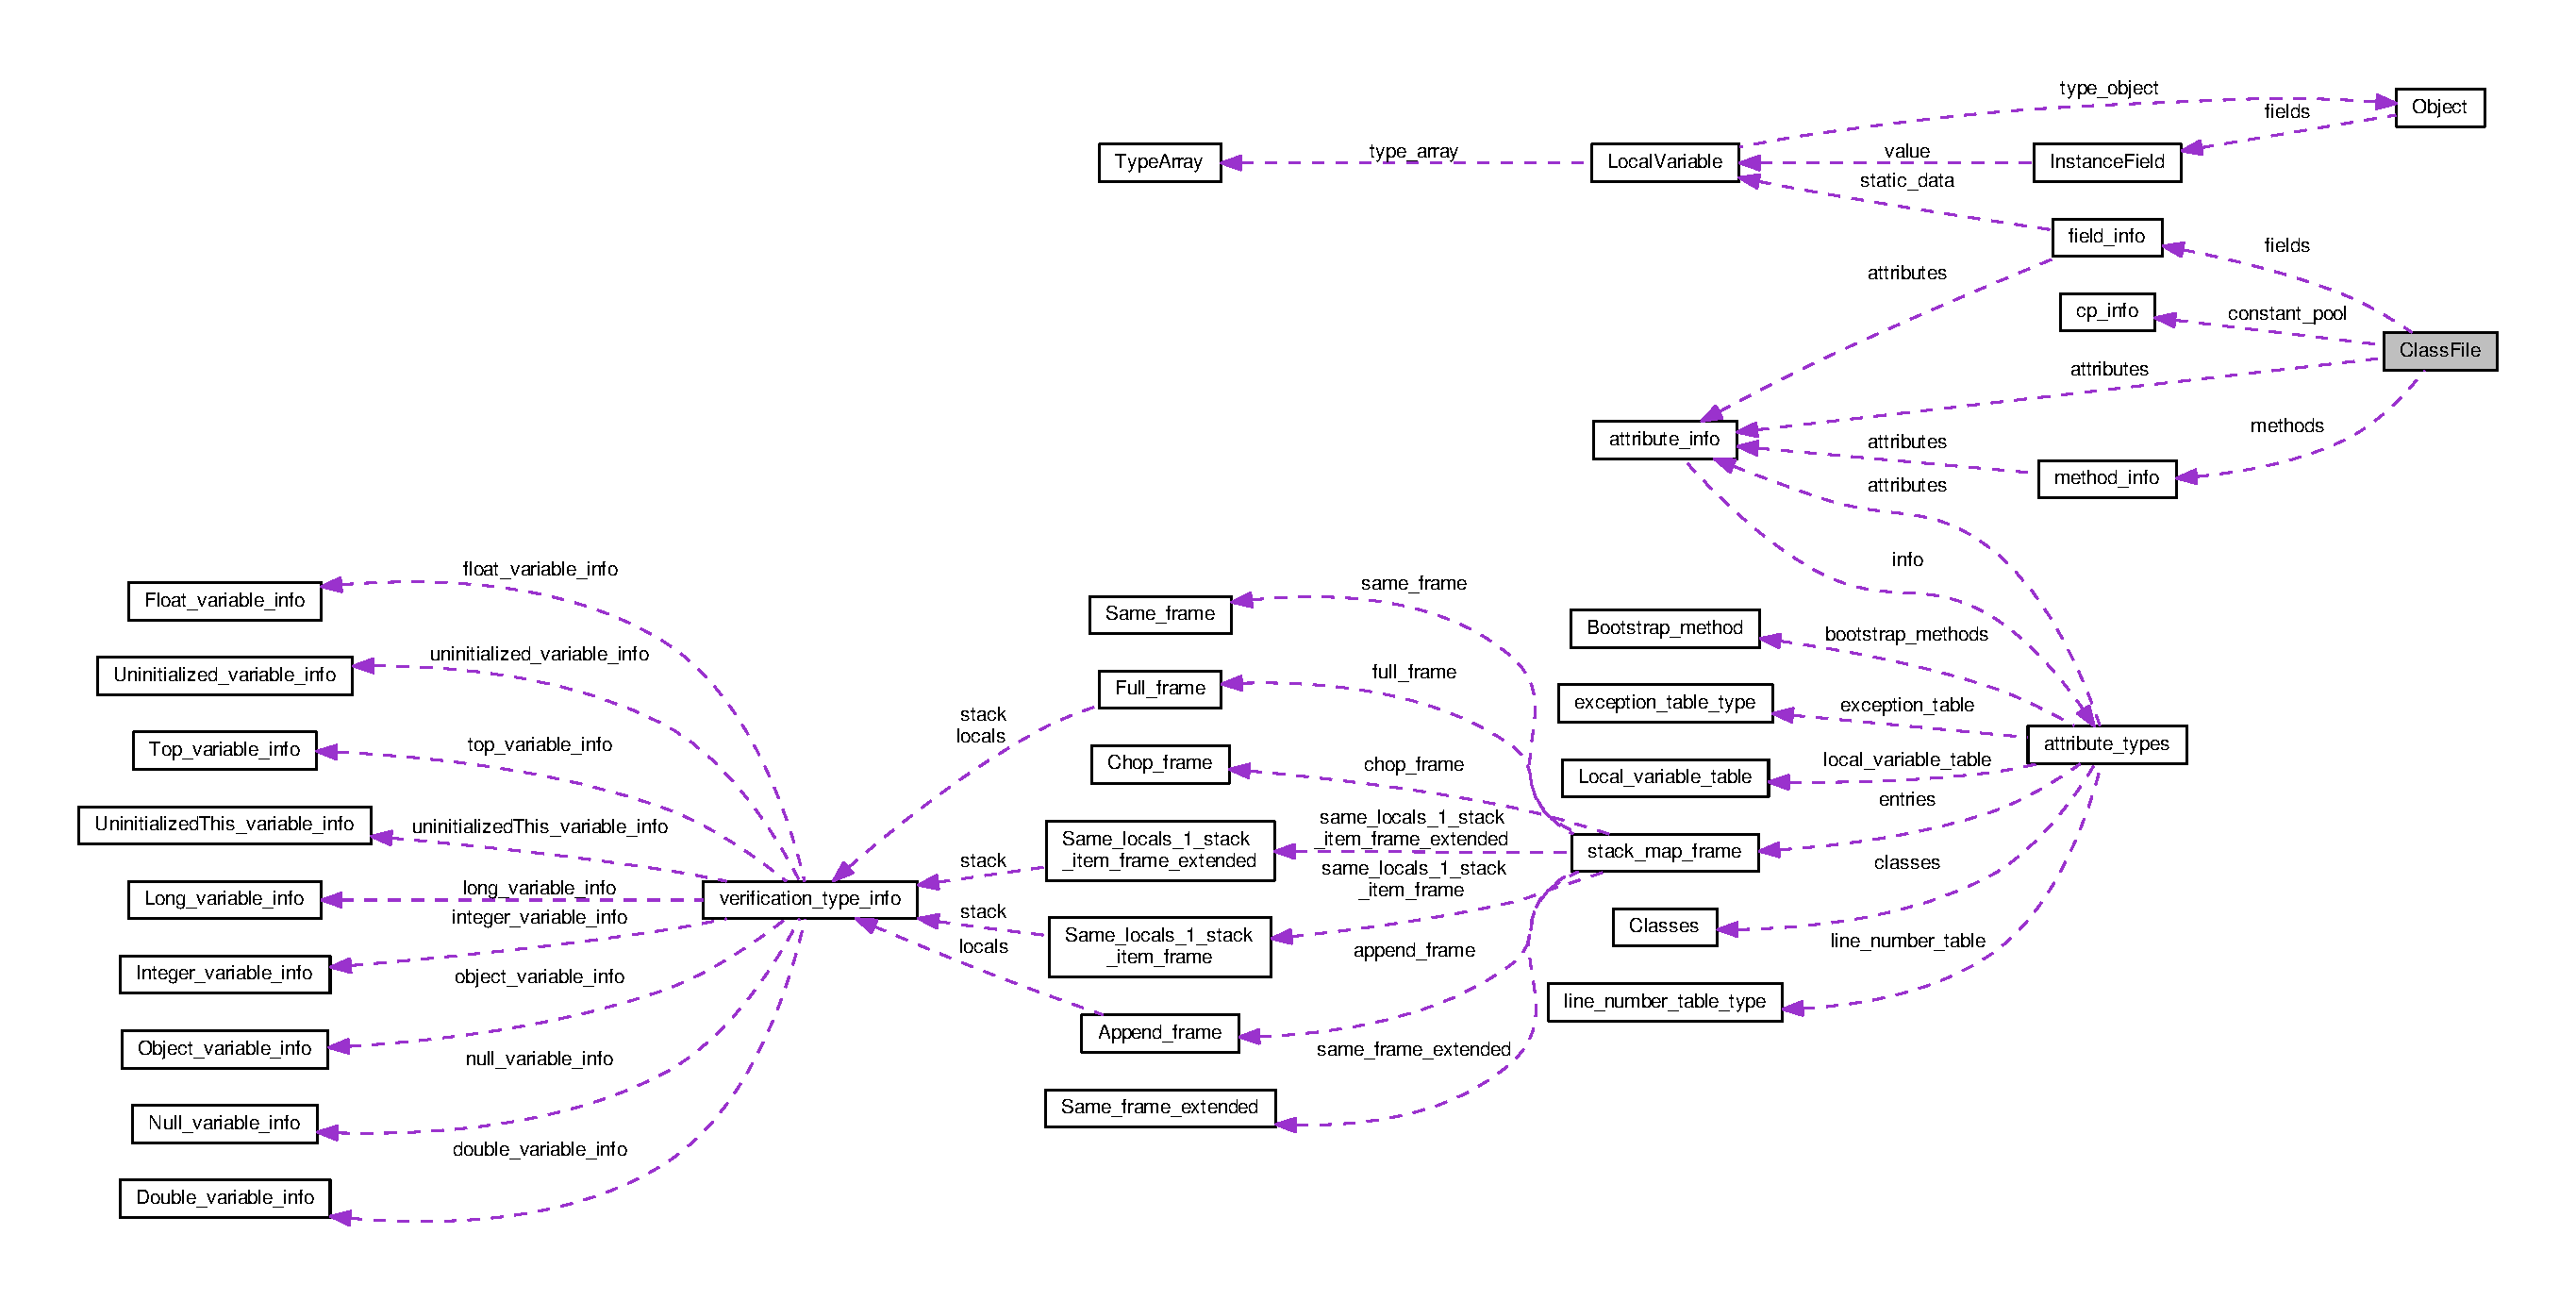
\includegraphics[width=350pt]{structClassFile__coll__graph}
\end{center}
\end{figure}
\subsection*{Public Attributes}
\begin{DoxyCompactItemize}
\item 
\hyperlink{structures_8h_ae391a1d79bb0c8cbc283f0283e3c098b}{u4} \hyperlink{structClassFile_a09085e9db513dae2f46da6e0a26c1b59}{magic}
\item 
\hyperlink{structures_8h_a55ef8d87fd202b8417704c089899c5b9}{u2} \hyperlink{structClassFile_af0db7b0ea01cb9cea2cee177ca81df09}{minor\+\_\+version}
\item 
\hyperlink{structures_8h_a55ef8d87fd202b8417704c089899c5b9}{u2} \hyperlink{structClassFile_abede9cb937e65072517d0ee6e26e2757}{major\+\_\+version}
\item 
\hyperlink{structures_8h_a55ef8d87fd202b8417704c089899c5b9}{u2} \hyperlink{structClassFile_ac8fdf5cccfd632da4fdb21ae63fffa7a}{constant\+\_\+pool\+\_\+count}
\item 
\hyperlink{structcp__info}{cp\+\_\+info} $\ast$ \hyperlink{structClassFile_a2309d843091aad79aed04ce92470a434}{constant\+\_\+pool}
\item 
\hyperlink{structures_8h_a55ef8d87fd202b8417704c089899c5b9}{u2} \hyperlink{structClassFile_ae88db578147f7ee0d6fc1aeacb341854}{access\+\_\+flags}
\item 
\hyperlink{structures_8h_a55ef8d87fd202b8417704c089899c5b9}{u2} \hyperlink{structClassFile_a2d33db0a560a71b94bc572dd1e4ec03a}{this\+\_\+class}
\item 
\hyperlink{structures_8h_a55ef8d87fd202b8417704c089899c5b9}{u2} \hyperlink{structClassFile_a5f6c11c0ccb02fd992b5c102725253ec}{super\+\_\+class}
\item 
\hyperlink{structures_8h_a55ef8d87fd202b8417704c089899c5b9}{u2} \hyperlink{structClassFile_a337fcb7da33d1b64631441115c7de305}{interfaces\+\_\+count}
\item 
\hyperlink{structures_8h_a55ef8d87fd202b8417704c089899c5b9}{u2} $\ast$ \hyperlink{structClassFile_af599de97e062c98966470f1590496425}{interfaces}
\item 
\hyperlink{structures_8h_a55ef8d87fd202b8417704c089899c5b9}{u2} \hyperlink{structClassFile_acea207ee523fbc16611d3cf436c390e0}{fields\+\_\+count}
\item 
\hyperlink{structfield__info}{field\+\_\+info} $\ast$ \hyperlink{structClassFile_aa324f88c75aa96c632f8c57d010aab0c}{fields}
\item 
\hyperlink{structures_8h_a55ef8d87fd202b8417704c089899c5b9}{u2} \hyperlink{structClassFile_aacfb45d4af64216324b1ae5269c870d5}{methods\+\_\+count}
\item 
\hyperlink{structmethod__info}{method\+\_\+info} $\ast$ \hyperlink{structClassFile_ad061f06cd709d10dbfbf82f443e43632}{methods}
\item 
\hyperlink{structures_8h_a55ef8d87fd202b8417704c089899c5b9}{u2} \hyperlink{structClassFile_a633c696fbe08e7e7906b2ab1e52f3d1b}{attributes\+\_\+count}
\item 
\hyperlink{structattribute__info}{attribute\+\_\+info} $\ast$ \hyperlink{structClassFile_a8bf809db8e1008f401dc3cda5e9cdb14}{attributes}
\end{DoxyCompactItemize}


\subsection{Detailed Description}
Struct que representa os campos do bytecode. 

Struct que representa o \hyperlink{structClassFile}{Class\+File}, para ser alocada pelo Class\+Loader e preenchida pela função \hyperlink{classfile_8c_a14c4d3f84dd03a43aca0a57bd530f3a2}{read\+\_\+class\+\_\+file()} 

\subsection{Member Data Documentation}
\index{Class\+File@{Class\+File}!access\+\_\+flags@{access\+\_\+flags}}
\index{access\+\_\+flags@{access\+\_\+flags}!Class\+File@{Class\+File}}
\subsubsection[{\texorpdfstring{access\+\_\+flags}{access_flags}}]{\setlength{\rightskip}{0pt plus 5cm}{\bf u2} Class\+File\+::access\+\_\+flags}\hypertarget{structClassFile_ae88db578147f7ee0d6fc1aeacb341854}{}\label{structClassFile_ae88db578147f7ee0d6fc1aeacb341854}
\index{Class\+File@{Class\+File}!attributes@{attributes}}
\index{attributes@{attributes}!Class\+File@{Class\+File}}
\subsubsection[{\texorpdfstring{attributes}{attributes}}]{\setlength{\rightskip}{0pt plus 5cm}{\bf attribute\+\_\+info}$\ast$ Class\+File\+::attributes}\hypertarget{structClassFile_a8bf809db8e1008f401dc3cda5e9cdb14}{}\label{structClassFile_a8bf809db8e1008f401dc3cda5e9cdb14}
\index{Class\+File@{Class\+File}!attributes\+\_\+count@{attributes\+\_\+count}}
\index{attributes\+\_\+count@{attributes\+\_\+count}!Class\+File@{Class\+File}}
\subsubsection[{\texorpdfstring{attributes\+\_\+count}{attributes_count}}]{\setlength{\rightskip}{0pt plus 5cm}{\bf u2} Class\+File\+::attributes\+\_\+count}\hypertarget{structClassFile_a633c696fbe08e7e7906b2ab1e52f3d1b}{}\label{structClassFile_a633c696fbe08e7e7906b2ab1e52f3d1b}
\index{Class\+File@{Class\+File}!constant\+\_\+pool@{constant\+\_\+pool}}
\index{constant\+\_\+pool@{constant\+\_\+pool}!Class\+File@{Class\+File}}
\subsubsection[{\texorpdfstring{constant\+\_\+pool}{constant_pool}}]{\setlength{\rightskip}{0pt plus 5cm}{\bf cp\+\_\+info}$\ast$ Class\+File\+::constant\+\_\+pool}\hypertarget{structClassFile_a2309d843091aad79aed04ce92470a434}{}\label{structClassFile_a2309d843091aad79aed04ce92470a434}
\index{Class\+File@{Class\+File}!constant\+\_\+pool\+\_\+count@{constant\+\_\+pool\+\_\+count}}
\index{constant\+\_\+pool\+\_\+count@{constant\+\_\+pool\+\_\+count}!Class\+File@{Class\+File}}
\subsubsection[{\texorpdfstring{constant\+\_\+pool\+\_\+count}{constant_pool_count}}]{\setlength{\rightskip}{0pt plus 5cm}{\bf u2} Class\+File\+::constant\+\_\+pool\+\_\+count}\hypertarget{structClassFile_ac8fdf5cccfd632da4fdb21ae63fffa7a}{}\label{structClassFile_ac8fdf5cccfd632da4fdb21ae63fffa7a}
\index{Class\+File@{Class\+File}!fields@{fields}}
\index{fields@{fields}!Class\+File@{Class\+File}}
\subsubsection[{\texorpdfstring{fields}{fields}}]{\setlength{\rightskip}{0pt plus 5cm}{\bf field\+\_\+info}$\ast$ Class\+File\+::fields}\hypertarget{structClassFile_aa324f88c75aa96c632f8c57d010aab0c}{}\label{structClassFile_aa324f88c75aa96c632f8c57d010aab0c}
\index{Class\+File@{Class\+File}!fields\+\_\+count@{fields\+\_\+count}}
\index{fields\+\_\+count@{fields\+\_\+count}!Class\+File@{Class\+File}}
\subsubsection[{\texorpdfstring{fields\+\_\+count}{fields_count}}]{\setlength{\rightskip}{0pt plus 5cm}{\bf u2} Class\+File\+::fields\+\_\+count}\hypertarget{structClassFile_acea207ee523fbc16611d3cf436c390e0}{}\label{structClassFile_acea207ee523fbc16611d3cf436c390e0}
\index{Class\+File@{Class\+File}!interfaces@{interfaces}}
\index{interfaces@{interfaces}!Class\+File@{Class\+File}}
\subsubsection[{\texorpdfstring{interfaces}{interfaces}}]{\setlength{\rightskip}{0pt plus 5cm}{\bf u2}$\ast$ Class\+File\+::interfaces}\hypertarget{structClassFile_af599de97e062c98966470f1590496425}{}\label{structClassFile_af599de97e062c98966470f1590496425}
\index{Class\+File@{Class\+File}!interfaces\+\_\+count@{interfaces\+\_\+count}}
\index{interfaces\+\_\+count@{interfaces\+\_\+count}!Class\+File@{Class\+File}}
\subsubsection[{\texorpdfstring{interfaces\+\_\+count}{interfaces_count}}]{\setlength{\rightskip}{0pt plus 5cm}{\bf u2} Class\+File\+::interfaces\+\_\+count}\hypertarget{structClassFile_a337fcb7da33d1b64631441115c7de305}{}\label{structClassFile_a337fcb7da33d1b64631441115c7de305}
\index{Class\+File@{Class\+File}!magic@{magic}}
\index{magic@{magic}!Class\+File@{Class\+File}}
\subsubsection[{\texorpdfstring{magic}{magic}}]{\setlength{\rightskip}{0pt plus 5cm}{\bf u4} Class\+File\+::magic}\hypertarget{structClassFile_a09085e9db513dae2f46da6e0a26c1b59}{}\label{structClassFile_a09085e9db513dae2f46da6e0a26c1b59}
\index{Class\+File@{Class\+File}!major\+\_\+version@{major\+\_\+version}}
\index{major\+\_\+version@{major\+\_\+version}!Class\+File@{Class\+File}}
\subsubsection[{\texorpdfstring{major\+\_\+version}{major_version}}]{\setlength{\rightskip}{0pt plus 5cm}{\bf u2} Class\+File\+::major\+\_\+version}\hypertarget{structClassFile_abede9cb937e65072517d0ee6e26e2757}{}\label{structClassFile_abede9cb937e65072517d0ee6e26e2757}
\index{Class\+File@{Class\+File}!methods@{methods}}
\index{methods@{methods}!Class\+File@{Class\+File}}
\subsubsection[{\texorpdfstring{methods}{methods}}]{\setlength{\rightskip}{0pt plus 5cm}{\bf method\+\_\+info}$\ast$ Class\+File\+::methods}\hypertarget{structClassFile_ad061f06cd709d10dbfbf82f443e43632}{}\label{structClassFile_ad061f06cd709d10dbfbf82f443e43632}
\index{Class\+File@{Class\+File}!methods\+\_\+count@{methods\+\_\+count}}
\index{methods\+\_\+count@{methods\+\_\+count}!Class\+File@{Class\+File}}
\subsubsection[{\texorpdfstring{methods\+\_\+count}{methods_count}}]{\setlength{\rightskip}{0pt plus 5cm}{\bf u2} Class\+File\+::methods\+\_\+count}\hypertarget{structClassFile_aacfb45d4af64216324b1ae5269c870d5}{}\label{structClassFile_aacfb45d4af64216324b1ae5269c870d5}
\index{Class\+File@{Class\+File}!minor\+\_\+version@{minor\+\_\+version}}
\index{minor\+\_\+version@{minor\+\_\+version}!Class\+File@{Class\+File}}
\subsubsection[{\texorpdfstring{minor\+\_\+version}{minor_version}}]{\setlength{\rightskip}{0pt plus 5cm}{\bf u2} Class\+File\+::minor\+\_\+version}\hypertarget{structClassFile_af0db7b0ea01cb9cea2cee177ca81df09}{}\label{structClassFile_af0db7b0ea01cb9cea2cee177ca81df09}
\index{Class\+File@{Class\+File}!super\+\_\+class@{super\+\_\+class}}
\index{super\+\_\+class@{super\+\_\+class}!Class\+File@{Class\+File}}
\subsubsection[{\texorpdfstring{super\+\_\+class}{super_class}}]{\setlength{\rightskip}{0pt plus 5cm}{\bf u2} Class\+File\+::super\+\_\+class}\hypertarget{structClassFile_a5f6c11c0ccb02fd992b5c102725253ec}{}\label{structClassFile_a5f6c11c0ccb02fd992b5c102725253ec}
\index{Class\+File@{Class\+File}!this\+\_\+class@{this\+\_\+class}}
\index{this\+\_\+class@{this\+\_\+class}!Class\+File@{Class\+File}}
\subsubsection[{\texorpdfstring{this\+\_\+class}{this_class}}]{\setlength{\rightskip}{0pt plus 5cm}{\bf u2} Class\+File\+::this\+\_\+class}\hypertarget{structClassFile_a2d33db0a560a71b94bc572dd1e4ec03a}{}\label{structClassFile_a2d33db0a560a71b94bc572dd1e4ec03a}


The documentation for this struct was generated from the following file\+:\begin{DoxyCompactItemize}
\item 
\hyperlink{structures_8h}{structures.\+h}\end{DoxyCompactItemize}

\hypertarget{structcp__info}{}\section{cp\+\_\+info Struct Reference}
\label{structcp__info}\index{cp\+\_\+info@{cp\+\_\+info}}


{\ttfamily \#include $<$structures.\+h$>$}

\subsection*{Public Attributes}
\begin{DoxyCompactItemize}
\item 
\hyperlink{structures_8h_a64f8055b64cf2a4c299c841130c5c938}{u1} \hyperlink{structcp__info_a045b8801a6e96a2a31d3b62ea684f141}{tag}
\item 
\begin{tabbing}
xx\=xx\=xx\=xx\=xx\=xx\=xx\=xx\=xx\=\kill
union \{\\
\>struct \{\\
\>\>\hyperlink{structures_8h_a55ef8d87fd202b8417704c089899c5b9}{u2} \hyperlink{structcp__info_a0b2c4677d0d56defd858fdc796caec87}{name\_index}\\
\>\} \hyperlink{structcp__info_a322117cc9b35710232212d96443b9c46}{Class}\\
\>struct \{\\
\>\>\hyperlink{structures_8h_a55ef8d87fd202b8417704c089899c5b9}{u2} \hyperlink{structcp__info_a1c7c3f3e2f9a620669b5f5cc51249ef8}{class\_index}\\
\>\>\hyperlink{structures_8h_a55ef8d87fd202b8417704c089899c5b9}{u2} \hyperlink{structcp__info_a1b947f3ff3eee58acf5500debf45848c}{name\_and\_type\_index}\\
\>\} \hyperlink{structcp__info_aee4742a1bbb698a449a95a88dfc6b4f9}{Fieldref}\\
\>struct \{\\
\>\>\hyperlink{structures_8h_a55ef8d87fd202b8417704c089899c5b9}{u2} \hyperlink{structcp__info_a1c7c3f3e2f9a620669b5f5cc51249ef8}{class\_index}\\
\>\>\hyperlink{structures_8h_a55ef8d87fd202b8417704c089899c5b9}{u2} \hyperlink{structcp__info_a1b947f3ff3eee58acf5500debf45848c}{name\_and\_type\_index}\\
\>\} \hyperlink{structcp__info_ae02638b6c90e9d24eae9c8bfc4b09f1c}{Methodref}\\
\>struct \{\\
\>\>\hyperlink{structures_8h_a55ef8d87fd202b8417704c089899c5b9}{u2} \hyperlink{structcp__info_a1c7c3f3e2f9a620669b5f5cc51249ef8}{class\_index}\\
\>\>\hyperlink{structures_8h_a55ef8d87fd202b8417704c089899c5b9}{u2} \hyperlink{structcp__info_a1b947f3ff3eee58acf5500debf45848c}{name\_and\_type\_index}\\
\>\} \hyperlink{structcp__info_a4bc2525cea570eff1133480f351ab833}{InterfaceMethodref}\\
\>struct \{\\
\>\>\hyperlink{structures_8h_a55ef8d87fd202b8417704c089899c5b9}{u2} \hyperlink{structcp__info_ae760e12a2ee01b0ace3d35170ca07981}{string\_index}\\
\>\} \hyperlink{structcp__info_a453cf965166c542ff75a14db651769e3}{String}\\
\>struct \{\\
\>\>\hyperlink{structures_8h_ae391a1d79bb0c8cbc283f0283e3c098b}{u4} \hyperlink{structcp__info_a4dcce18f4a19e8112079dc11dc2f5386}{bytes}\\
\>\} \hyperlink{structcp__info_ada2bb1a48d398e9ecaf3180eb82bbd32}{Integer}\\
\>struct \{\\
\>\>\hyperlink{structures_8h_ae391a1d79bb0c8cbc283f0283e3c098b}{u4} \hyperlink{structcp__info_a4dcce18f4a19e8112079dc11dc2f5386}{bytes}\\
\>\} \hyperlink{structcp__info_ae1a57be30f86f89552e556c01a186461}{Float}\\
\>struct \{\\
\>\>\hyperlink{structures_8h_ae391a1d79bb0c8cbc283f0283e3c098b}{u4} \hyperlink{structcp__info_a26996f9b4a0caab37c9cdbfd027eaed7}{high\_bytes}\\
\>\>\hyperlink{structures_8h_ae391a1d79bb0c8cbc283f0283e3c098b}{u4} \hyperlink{structcp__info_aff872b9dcff18e083ca9f73ef82ab14f}{low\_bytes}\\
\>\} \hyperlink{structcp__info_aaef6412a3f5c1011817df7889b13461d}{Long}\\
\>struct \{\\
\>\>\hyperlink{structures_8h_ae391a1d79bb0c8cbc283f0283e3c098b}{u4} \hyperlink{structcp__info_a26996f9b4a0caab37c9cdbfd027eaed7}{high\_bytes}\\
\>\>\hyperlink{structures_8h_ae391a1d79bb0c8cbc283f0283e3c098b}{u4} \hyperlink{structcp__info_aff872b9dcff18e083ca9f73ef82ab14f}{low\_bytes}\\
\>\} \hyperlink{structcp__info_ac501a57eed33b25313614096d0b2d80c}{Double}\\
\>struct \{\\
\>\>\hyperlink{structures_8h_a55ef8d87fd202b8417704c089899c5b9}{u2} \hyperlink{structcp__info_a0b2c4677d0d56defd858fdc796caec87}{name\_index}\\
\>\>\hyperlink{structures_8h_a55ef8d87fd202b8417704c089899c5b9}{u2} \hyperlink{structcp__info_a35ec31f117bf83ef9aef6100822f1141}{descriptor\_index}\\
\>\} \hyperlink{structcp__info_ac43e804549f01bed269b46ac2fd0efca}{NameAndType}\\
\>struct \{\\
\>\>\hyperlink{structures_8h_a55ef8d87fd202b8417704c089899c5b9}{u2} \hyperlink{structcp__info_a1df458be110c843ea49b8a8a4c9dfb91}{length}\\
\>\>\hyperlink{structures_8h_a64f8055b64cf2a4c299c841130c5c938}{u1} $\ast$ \hyperlink{structcp__info_a30f97eda54e30a923a217520316e9301}{bytes}\\
\>\} \hyperlink{structcp__info_af0b0a05e0079e3d1b0c99cd3c0e4463a}{Utf8}\\
\>struct \{\\
\>\>\hyperlink{structures_8h_a64f8055b64cf2a4c299c841130c5c938}{u1} \hyperlink{structcp__info_a13e5aa07b7aa482061b89f4d7379a2dd}{reference\_kind}\\
\>\>\hyperlink{structures_8h_a55ef8d87fd202b8417704c089899c5b9}{u2} \hyperlink{structcp__info_a946bbab9aa280d4e22194ef7b434166a}{reference\_index}\\
\>\} \hyperlink{structcp__info_a6a4f93d961e65bc33c079ba656b89884}{MethodHandle}\\
\>struct \{\\
\>\>\hyperlink{structures_8h_a55ef8d87fd202b8417704c089899c5b9}{u2} \hyperlink{structcp__info_a35ec31f117bf83ef9aef6100822f1141}{descriptor\_index}\\
\>\} \hyperlink{structcp__info_a2faf7cea4242acbc5f952567fdabfb72}{MethodType}\\
\>struct \{\\
\>\>\hyperlink{structures_8h_a55ef8d87fd202b8417704c089899c5b9}{u2} \hyperlink{structcp__info_abad11f89efc244065e72ec811f9dc929}{bootstrap\_method\_attr\_index}\\
\>\>\hyperlink{structures_8h_a55ef8d87fd202b8417704c089899c5b9}{u2} \hyperlink{structcp__info_a1b947f3ff3eee58acf5500debf45848c}{name\_and\_type\_index}\\
\>\} \hyperlink{structcp__info_a9f368f50ec505be7deadf4af55074cdd}{InvokeDynamic}\\
\}; \\

\end{tabbing}\end{DoxyCompactItemize}


\subsection{Detailed Description}
Struct para indicar o tipo de constant\+\_\+pool (tendo uma tag associada e mais atributos em função da constante)

Union\+: serve para alocar espaço pra maior struct 

\subsection{Member Data Documentation}
\subsubsection[{\texorpdfstring{"@5}{@5}}]{\setlength{\rightskip}{0pt plus 5cm}union \{ ... \} }\hypertarget{structcp__info_a0469358e891d5c89038d59f1807d00b2}{}\label{structcp__info_a0469358e891d5c89038d59f1807d00b2}
\index{cp\+\_\+info@{cp\+\_\+info}!bootstrap\+\_\+method\+\_\+attr\+\_\+index@{bootstrap\+\_\+method\+\_\+attr\+\_\+index}}
\index{bootstrap\+\_\+method\+\_\+attr\+\_\+index@{bootstrap\+\_\+method\+\_\+attr\+\_\+index}!cp\+\_\+info@{cp\+\_\+info}}
\subsubsection[{\texorpdfstring{bootstrap\+\_\+method\+\_\+attr\+\_\+index}{bootstrap_method_attr_index}}]{\setlength{\rightskip}{0pt plus 5cm}{\bf u2} cp\+\_\+info\+::bootstrap\+\_\+method\+\_\+attr\+\_\+index}\hypertarget{structcp__info_abad11f89efc244065e72ec811f9dc929}{}\label{structcp__info_abad11f89efc244065e72ec811f9dc929}
\index{cp\+\_\+info@{cp\+\_\+info}!bytes@{bytes}}
\index{bytes@{bytes}!cp\+\_\+info@{cp\+\_\+info}}
\subsubsection[{\texorpdfstring{bytes}{bytes}}]{\setlength{\rightskip}{0pt plus 5cm}{\bf u4} cp\+\_\+info\+::bytes}\hypertarget{structcp__info_a4dcce18f4a19e8112079dc11dc2f5386}{}\label{structcp__info_a4dcce18f4a19e8112079dc11dc2f5386}
\index{cp\+\_\+info@{cp\+\_\+info}!bytes@{bytes}}
\index{bytes@{bytes}!cp\+\_\+info@{cp\+\_\+info}}
\subsubsection[{\texorpdfstring{bytes}{bytes}}]{\setlength{\rightskip}{0pt plus 5cm}{\bf u1}$\ast$ cp\+\_\+info\+::bytes}\hypertarget{structcp__info_a30f97eda54e30a923a217520316e9301}{}\label{structcp__info_a30f97eda54e30a923a217520316e9301}
\index{cp\+\_\+info@{cp\+\_\+info}!Class@{Class}}
\index{Class@{Class}!cp\+\_\+info@{cp\+\_\+info}}
\subsubsection[{\texorpdfstring{Class}{Class}}]{\setlength{\rightskip}{0pt plus 5cm}struct \{ ... \}   cp\+\_\+info\+::\+Class}\hypertarget{structcp__info_a322117cc9b35710232212d96443b9c46}{}\label{structcp__info_a322117cc9b35710232212d96443b9c46}
\index{cp\+\_\+info@{cp\+\_\+info}!class\+\_\+index@{class\+\_\+index}}
\index{class\+\_\+index@{class\+\_\+index}!cp\+\_\+info@{cp\+\_\+info}}
\subsubsection[{\texorpdfstring{class\+\_\+index}{class_index}}]{\setlength{\rightskip}{0pt plus 5cm}{\bf u2} cp\+\_\+info\+::class\+\_\+index}\hypertarget{structcp__info_a1c7c3f3e2f9a620669b5f5cc51249ef8}{}\label{structcp__info_a1c7c3f3e2f9a620669b5f5cc51249ef8}
\index{cp\+\_\+info@{cp\+\_\+info}!descriptor\+\_\+index@{descriptor\+\_\+index}}
\index{descriptor\+\_\+index@{descriptor\+\_\+index}!cp\+\_\+info@{cp\+\_\+info}}
\subsubsection[{\texorpdfstring{descriptor\+\_\+index}{descriptor_index}}]{\setlength{\rightskip}{0pt plus 5cm}{\bf u2} cp\+\_\+info\+::descriptor\+\_\+index}\hypertarget{structcp__info_a35ec31f117bf83ef9aef6100822f1141}{}\label{structcp__info_a35ec31f117bf83ef9aef6100822f1141}
\index{cp\+\_\+info@{cp\+\_\+info}!Double@{Double}}
\index{Double@{Double}!cp\+\_\+info@{cp\+\_\+info}}
\subsubsection[{\texorpdfstring{Double}{Double}}]{\setlength{\rightskip}{0pt plus 5cm}struct \{ ... \}   cp\+\_\+info\+::\+Double}\hypertarget{structcp__info_ac501a57eed33b25313614096d0b2d80c}{}\label{structcp__info_ac501a57eed33b25313614096d0b2d80c}
\index{cp\+\_\+info@{cp\+\_\+info}!Fieldref@{Fieldref}}
\index{Fieldref@{Fieldref}!cp\+\_\+info@{cp\+\_\+info}}
\subsubsection[{\texorpdfstring{Fieldref}{Fieldref}}]{\setlength{\rightskip}{0pt plus 5cm}struct \{ ... \}   cp\+\_\+info\+::\+Fieldref}\hypertarget{structcp__info_aee4742a1bbb698a449a95a88dfc6b4f9}{}\label{structcp__info_aee4742a1bbb698a449a95a88dfc6b4f9}
\index{cp\+\_\+info@{cp\+\_\+info}!Float@{Float}}
\index{Float@{Float}!cp\+\_\+info@{cp\+\_\+info}}
\subsubsection[{\texorpdfstring{Float}{Float}}]{\setlength{\rightskip}{0pt plus 5cm}struct \{ ... \}   cp\+\_\+info\+::\+Float}\hypertarget{structcp__info_ae1a57be30f86f89552e556c01a186461}{}\label{structcp__info_ae1a57be30f86f89552e556c01a186461}
\index{cp\+\_\+info@{cp\+\_\+info}!high\+\_\+bytes@{high\+\_\+bytes}}
\index{high\+\_\+bytes@{high\+\_\+bytes}!cp\+\_\+info@{cp\+\_\+info}}
\subsubsection[{\texorpdfstring{high\+\_\+bytes}{high_bytes}}]{\setlength{\rightskip}{0pt plus 5cm}{\bf u4} cp\+\_\+info\+::high\+\_\+bytes}\hypertarget{structcp__info_a26996f9b4a0caab37c9cdbfd027eaed7}{}\label{structcp__info_a26996f9b4a0caab37c9cdbfd027eaed7}
\index{cp\+\_\+info@{cp\+\_\+info}!Integer@{Integer}}
\index{Integer@{Integer}!cp\+\_\+info@{cp\+\_\+info}}
\subsubsection[{\texorpdfstring{Integer}{Integer}}]{\setlength{\rightskip}{0pt plus 5cm}struct \{ ... \}   cp\+\_\+info\+::\+Integer}\hypertarget{structcp__info_ada2bb1a48d398e9ecaf3180eb82bbd32}{}\label{structcp__info_ada2bb1a48d398e9ecaf3180eb82bbd32}
\index{cp\+\_\+info@{cp\+\_\+info}!Interface\+Methodref@{Interface\+Methodref}}
\index{Interface\+Methodref@{Interface\+Methodref}!cp\+\_\+info@{cp\+\_\+info}}
\subsubsection[{\texorpdfstring{Interface\+Methodref}{InterfaceMethodref}}]{\setlength{\rightskip}{0pt plus 5cm}struct \{ ... \}   cp\+\_\+info\+::\+Interface\+Methodref}\hypertarget{structcp__info_a4bc2525cea570eff1133480f351ab833}{}\label{structcp__info_a4bc2525cea570eff1133480f351ab833}
\index{cp\+\_\+info@{cp\+\_\+info}!Invoke\+Dynamic@{Invoke\+Dynamic}}
\index{Invoke\+Dynamic@{Invoke\+Dynamic}!cp\+\_\+info@{cp\+\_\+info}}
\subsubsection[{\texorpdfstring{Invoke\+Dynamic}{InvokeDynamic}}]{\setlength{\rightskip}{0pt plus 5cm}struct \{ ... \}   cp\+\_\+info\+::\+Invoke\+Dynamic}\hypertarget{structcp__info_a9f368f50ec505be7deadf4af55074cdd}{}\label{structcp__info_a9f368f50ec505be7deadf4af55074cdd}
\index{cp\+\_\+info@{cp\+\_\+info}!length@{length}}
\index{length@{length}!cp\+\_\+info@{cp\+\_\+info}}
\subsubsection[{\texorpdfstring{length}{length}}]{\setlength{\rightskip}{0pt plus 5cm}{\bf u2} cp\+\_\+info\+::length}\hypertarget{structcp__info_a1df458be110c843ea49b8a8a4c9dfb91}{}\label{structcp__info_a1df458be110c843ea49b8a8a4c9dfb91}
\index{cp\+\_\+info@{cp\+\_\+info}!Long@{Long}}
\index{Long@{Long}!cp\+\_\+info@{cp\+\_\+info}}
\subsubsection[{\texorpdfstring{Long}{Long}}]{\setlength{\rightskip}{0pt plus 5cm}struct \{ ... \}   cp\+\_\+info\+::\+Long}\hypertarget{structcp__info_aaef6412a3f5c1011817df7889b13461d}{}\label{structcp__info_aaef6412a3f5c1011817df7889b13461d}
\index{cp\+\_\+info@{cp\+\_\+info}!low\+\_\+bytes@{low\+\_\+bytes}}
\index{low\+\_\+bytes@{low\+\_\+bytes}!cp\+\_\+info@{cp\+\_\+info}}
\subsubsection[{\texorpdfstring{low\+\_\+bytes}{low_bytes}}]{\setlength{\rightskip}{0pt plus 5cm}{\bf u4} cp\+\_\+info\+::low\+\_\+bytes}\hypertarget{structcp__info_aff872b9dcff18e083ca9f73ef82ab14f}{}\label{structcp__info_aff872b9dcff18e083ca9f73ef82ab14f}
\index{cp\+\_\+info@{cp\+\_\+info}!Method\+Handle@{Method\+Handle}}
\index{Method\+Handle@{Method\+Handle}!cp\+\_\+info@{cp\+\_\+info}}
\subsubsection[{\texorpdfstring{Method\+Handle}{MethodHandle}}]{\setlength{\rightskip}{0pt plus 5cm}struct \{ ... \}   cp\+\_\+info\+::\+Method\+Handle}\hypertarget{structcp__info_a6a4f93d961e65bc33c079ba656b89884}{}\label{structcp__info_a6a4f93d961e65bc33c079ba656b89884}
\index{cp\+\_\+info@{cp\+\_\+info}!Methodref@{Methodref}}
\index{Methodref@{Methodref}!cp\+\_\+info@{cp\+\_\+info}}
\subsubsection[{\texorpdfstring{Methodref}{Methodref}}]{\setlength{\rightskip}{0pt plus 5cm}struct \{ ... \}   cp\+\_\+info\+::\+Methodref}\hypertarget{structcp__info_ae02638b6c90e9d24eae9c8bfc4b09f1c}{}\label{structcp__info_ae02638b6c90e9d24eae9c8bfc4b09f1c}
\index{cp\+\_\+info@{cp\+\_\+info}!Method\+Type@{Method\+Type}}
\index{Method\+Type@{Method\+Type}!cp\+\_\+info@{cp\+\_\+info}}
\subsubsection[{\texorpdfstring{Method\+Type}{MethodType}}]{\setlength{\rightskip}{0pt plus 5cm}struct \{ ... \}   cp\+\_\+info\+::\+Method\+Type}\hypertarget{structcp__info_a2faf7cea4242acbc5f952567fdabfb72}{}\label{structcp__info_a2faf7cea4242acbc5f952567fdabfb72}
\index{cp\+\_\+info@{cp\+\_\+info}!name\+\_\+and\+\_\+type\+\_\+index@{name\+\_\+and\+\_\+type\+\_\+index}}
\index{name\+\_\+and\+\_\+type\+\_\+index@{name\+\_\+and\+\_\+type\+\_\+index}!cp\+\_\+info@{cp\+\_\+info}}
\subsubsection[{\texorpdfstring{name\+\_\+and\+\_\+type\+\_\+index}{name_and_type_index}}]{\setlength{\rightskip}{0pt plus 5cm}{\bf u2} cp\+\_\+info\+::name\+\_\+and\+\_\+type\+\_\+index}\hypertarget{structcp__info_a1b947f3ff3eee58acf5500debf45848c}{}\label{structcp__info_a1b947f3ff3eee58acf5500debf45848c}
\index{cp\+\_\+info@{cp\+\_\+info}!name\+\_\+index@{name\+\_\+index}}
\index{name\+\_\+index@{name\+\_\+index}!cp\+\_\+info@{cp\+\_\+info}}
\subsubsection[{\texorpdfstring{name\+\_\+index}{name_index}}]{\setlength{\rightskip}{0pt plus 5cm}{\bf u2} cp\+\_\+info\+::name\+\_\+index}\hypertarget{structcp__info_a0b2c4677d0d56defd858fdc796caec87}{}\label{structcp__info_a0b2c4677d0d56defd858fdc796caec87}
\index{cp\+\_\+info@{cp\+\_\+info}!Name\+And\+Type@{Name\+And\+Type}}
\index{Name\+And\+Type@{Name\+And\+Type}!cp\+\_\+info@{cp\+\_\+info}}
\subsubsection[{\texorpdfstring{Name\+And\+Type}{NameAndType}}]{\setlength{\rightskip}{0pt plus 5cm}struct \{ ... \}   cp\+\_\+info\+::\+Name\+And\+Type}\hypertarget{structcp__info_ac43e804549f01bed269b46ac2fd0efca}{}\label{structcp__info_ac43e804549f01bed269b46ac2fd0efca}
\index{cp\+\_\+info@{cp\+\_\+info}!reference\+\_\+index@{reference\+\_\+index}}
\index{reference\+\_\+index@{reference\+\_\+index}!cp\+\_\+info@{cp\+\_\+info}}
\subsubsection[{\texorpdfstring{reference\+\_\+index}{reference_index}}]{\setlength{\rightskip}{0pt plus 5cm}{\bf u2} cp\+\_\+info\+::reference\+\_\+index}\hypertarget{structcp__info_a946bbab9aa280d4e22194ef7b434166a}{}\label{structcp__info_a946bbab9aa280d4e22194ef7b434166a}
\index{cp\+\_\+info@{cp\+\_\+info}!reference\+\_\+kind@{reference\+\_\+kind}}
\index{reference\+\_\+kind@{reference\+\_\+kind}!cp\+\_\+info@{cp\+\_\+info}}
\subsubsection[{\texorpdfstring{reference\+\_\+kind}{reference_kind}}]{\setlength{\rightskip}{0pt plus 5cm}{\bf u1} cp\+\_\+info\+::reference\+\_\+kind}\hypertarget{structcp__info_a13e5aa07b7aa482061b89f4d7379a2dd}{}\label{structcp__info_a13e5aa07b7aa482061b89f4d7379a2dd}
\index{cp\+\_\+info@{cp\+\_\+info}!String@{String}}
\index{String@{String}!cp\+\_\+info@{cp\+\_\+info}}
\subsubsection[{\texorpdfstring{String}{String}}]{\setlength{\rightskip}{0pt plus 5cm}struct \{ ... \}   cp\+\_\+info\+::\+String}\hypertarget{structcp__info_a453cf965166c542ff75a14db651769e3}{}\label{structcp__info_a453cf965166c542ff75a14db651769e3}
\index{cp\+\_\+info@{cp\+\_\+info}!string\+\_\+index@{string\+\_\+index}}
\index{string\+\_\+index@{string\+\_\+index}!cp\+\_\+info@{cp\+\_\+info}}
\subsubsection[{\texorpdfstring{string\+\_\+index}{string_index}}]{\setlength{\rightskip}{0pt plus 5cm}{\bf u2} cp\+\_\+info\+::string\+\_\+index}\hypertarget{structcp__info_ae760e12a2ee01b0ace3d35170ca07981}{}\label{structcp__info_ae760e12a2ee01b0ace3d35170ca07981}
\index{cp\+\_\+info@{cp\+\_\+info}!tag@{tag}}
\index{tag@{tag}!cp\+\_\+info@{cp\+\_\+info}}
\subsubsection[{\texorpdfstring{tag}{tag}}]{\setlength{\rightskip}{0pt plus 5cm}{\bf u1} cp\+\_\+info\+::tag}\hypertarget{structcp__info_a045b8801a6e96a2a31d3b62ea684f141}{}\label{structcp__info_a045b8801a6e96a2a31d3b62ea684f141}
\index{cp\+\_\+info@{cp\+\_\+info}!Utf8@{Utf8}}
\index{Utf8@{Utf8}!cp\+\_\+info@{cp\+\_\+info}}
\subsubsection[{\texorpdfstring{Utf8}{Utf8}}]{\setlength{\rightskip}{0pt plus 5cm}struct \{ ... \}   cp\+\_\+info\+::\+Utf8}\hypertarget{structcp__info_af0b0a05e0079e3d1b0c99cd3c0e4463a}{}\label{structcp__info_af0b0a05e0079e3d1b0c99cd3c0e4463a}


The documentation for this struct was generated from the following file\+:\begin{DoxyCompactItemize}
\item 
\hyperlink{structures_8h}{structures.\+h}\end{DoxyCompactItemize}

\hypertarget{structDouble__variable__info}{}\section{Double\+\_\+variable\+\_\+info Struct Reference}
\label{structDouble__variable__info}\index{Double\+\_\+variable\+\_\+info@{Double\+\_\+variable\+\_\+info}}


{\ttfamily \#include $<$structures.\+h$>$}



The documentation for this struct was generated from the following file\+:\begin{DoxyCompactItemize}
\item 
\hyperlink{structures_8h}{structures.\+h}\end{DoxyCompactItemize}

\hypertarget{structexception__table__type}{}\section{exception\+\_\+table\+\_\+type Struct Reference}
\label{structexception__table__type}\index{exception\+\_\+table\+\_\+type@{exception\+\_\+table\+\_\+type}}


{\ttfamily \#include $<$structures.\+h$>$}

\subsection*{Public Attributes}
\begin{DoxyCompactItemize}
\item 
\hyperlink{structures_8h_a55ef8d87fd202b8417704c089899c5b9}{u2} \hyperlink{structexception__table__type_a71cf8eaa3d06b89818100df6405b266d}{start\+\_\+pc}
\item 
\hyperlink{structures_8h_a55ef8d87fd202b8417704c089899c5b9}{u2} \hyperlink{structexception__table__type_a796565865a227dc76b0dd7c78e3f8424}{end\+\_\+pc}
\item 
\hyperlink{structures_8h_a55ef8d87fd202b8417704c089899c5b9}{u2} \hyperlink{structexception__table__type_af1b56d902850a41f63b7271029946759}{handler\+\_\+pc}
\item 
\hyperlink{structures_8h_a55ef8d87fd202b8417704c089899c5b9}{u2} \hyperlink{structexception__table__type_a663fa7b2d1a468b29913fd92e006a5dc}{catch\+\_\+type}
\end{DoxyCompactItemize}


\subsection{Member Data Documentation}
\index{exception\+\_\+table\+\_\+type@{exception\+\_\+table\+\_\+type}!catch\+\_\+type@{catch\+\_\+type}}
\index{catch\+\_\+type@{catch\+\_\+type}!exception\+\_\+table\+\_\+type@{exception\+\_\+table\+\_\+type}}
\subsubsection[{\texorpdfstring{catch\+\_\+type}{catch_type}}]{\setlength{\rightskip}{0pt plus 5cm}{\bf u2} exception\+\_\+table\+\_\+type\+::catch\+\_\+type}\hypertarget{structexception__table__type_a663fa7b2d1a468b29913fd92e006a5dc}{}\label{structexception__table__type_a663fa7b2d1a468b29913fd92e006a5dc}
\index{exception\+\_\+table\+\_\+type@{exception\+\_\+table\+\_\+type}!end\+\_\+pc@{end\+\_\+pc}}
\index{end\+\_\+pc@{end\+\_\+pc}!exception\+\_\+table\+\_\+type@{exception\+\_\+table\+\_\+type}}
\subsubsection[{\texorpdfstring{end\+\_\+pc}{end_pc}}]{\setlength{\rightskip}{0pt plus 5cm}{\bf u2} exception\+\_\+table\+\_\+type\+::end\+\_\+pc}\hypertarget{structexception__table__type_a796565865a227dc76b0dd7c78e3f8424}{}\label{structexception__table__type_a796565865a227dc76b0dd7c78e3f8424}
\index{exception\+\_\+table\+\_\+type@{exception\+\_\+table\+\_\+type}!handler\+\_\+pc@{handler\+\_\+pc}}
\index{handler\+\_\+pc@{handler\+\_\+pc}!exception\+\_\+table\+\_\+type@{exception\+\_\+table\+\_\+type}}
\subsubsection[{\texorpdfstring{handler\+\_\+pc}{handler_pc}}]{\setlength{\rightskip}{0pt plus 5cm}{\bf u2} exception\+\_\+table\+\_\+type\+::handler\+\_\+pc}\hypertarget{structexception__table__type_af1b56d902850a41f63b7271029946759}{}\label{structexception__table__type_af1b56d902850a41f63b7271029946759}
\index{exception\+\_\+table\+\_\+type@{exception\+\_\+table\+\_\+type}!start\+\_\+pc@{start\+\_\+pc}}
\index{start\+\_\+pc@{start\+\_\+pc}!exception\+\_\+table\+\_\+type@{exception\+\_\+table\+\_\+type}}
\subsubsection[{\texorpdfstring{start\+\_\+pc}{start_pc}}]{\setlength{\rightskip}{0pt plus 5cm}{\bf u2} exception\+\_\+table\+\_\+type\+::start\+\_\+pc}\hypertarget{structexception__table__type_a71cf8eaa3d06b89818100df6405b266d}{}\label{structexception__table__type_a71cf8eaa3d06b89818100df6405b266d}


The documentation for this struct was generated from the following file\+:\begin{DoxyCompactItemize}
\item 
\hyperlink{structures_8h}{structures.\+h}\end{DoxyCompactItemize}

\hypertarget{structfield__info}{}\section{field\+\_\+info Struct Reference}
\label{structfield__info}\index{field\+\_\+info@{field\+\_\+info}}


{\ttfamily \#include $<$structures.\+h$>$}



Collaboration diagram for field\+\_\+info\+:
\nopagebreak
\begin{figure}[H]
\begin{center}
\leavevmode
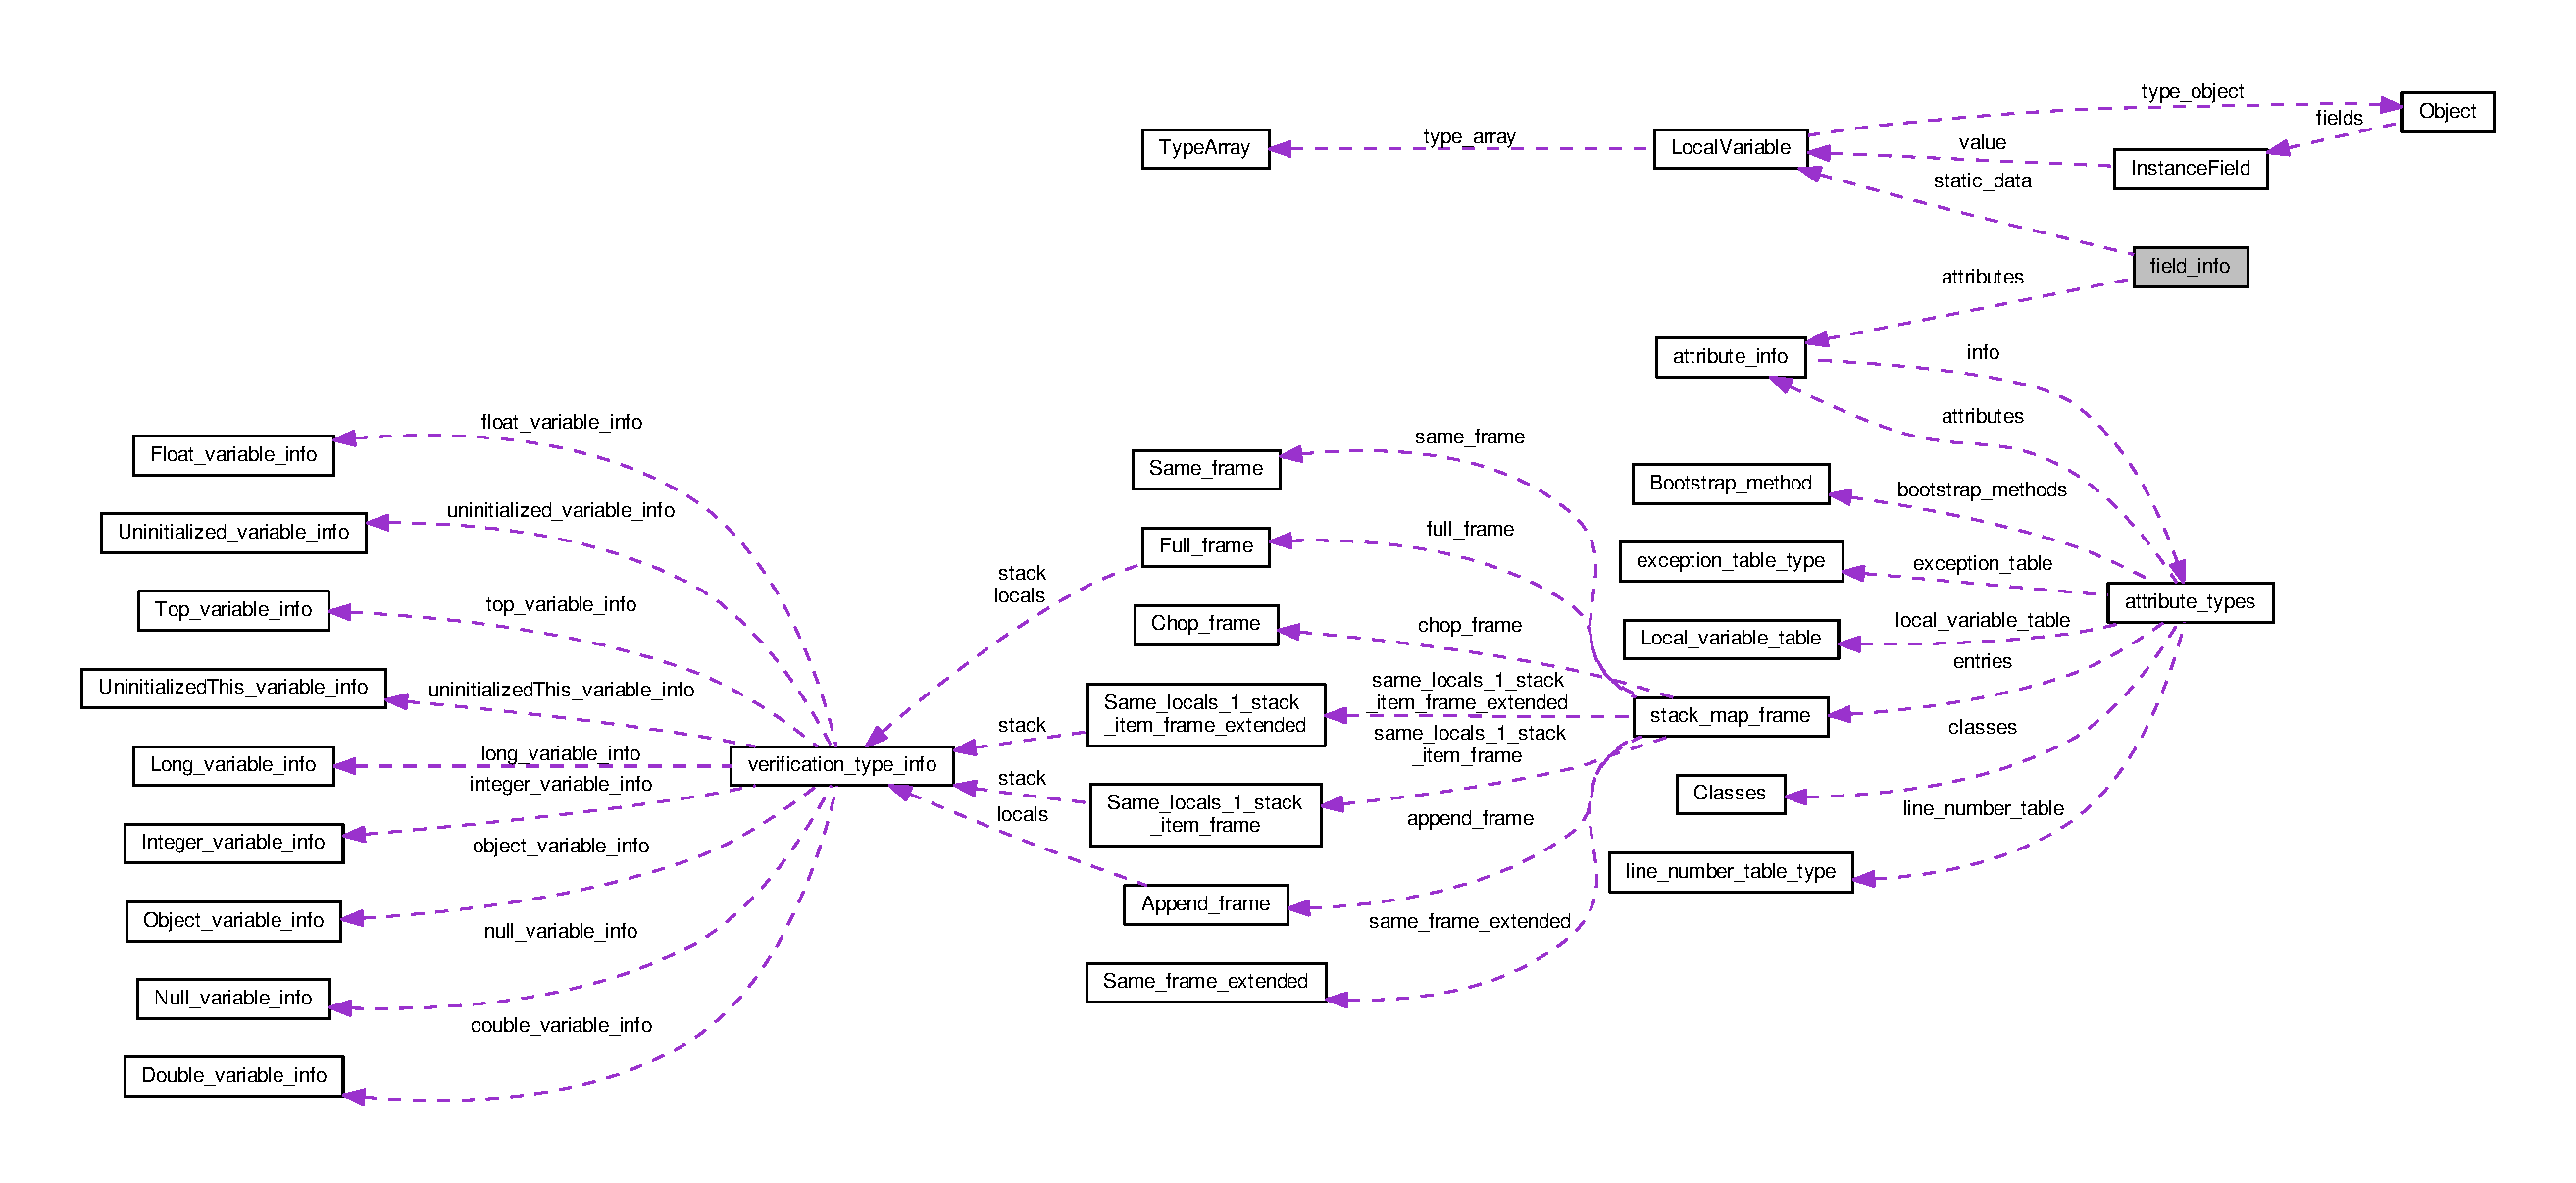
\includegraphics[width=350pt]{structfield__info__coll__graph}
\end{center}
\end{figure}
\subsection*{Public Attributes}
\begin{DoxyCompactItemize}
\item 
\hyperlink{structures_8h_a55ef8d87fd202b8417704c089899c5b9}{u2} \hyperlink{structfield__info_aa622dc9a5b5353d2f3eb2f416dacab4b}{access\+\_\+flags}
\item 
\hyperlink{structures_8h_a55ef8d87fd202b8417704c089899c5b9}{u2} \hyperlink{structfield__info_a425e3ae85badd81c67ef00acca85ad9e}{name\+\_\+index}
\item 
\hyperlink{structures_8h_a55ef8d87fd202b8417704c089899c5b9}{u2} \hyperlink{structfield__info_a12dd492b7fb1d61da1ac14938d97b07f}{descriptor\+\_\+index}
\item 
\hyperlink{structures_8h_a55ef8d87fd202b8417704c089899c5b9}{u2} \hyperlink{structfield__info_a83bfa4ff84a608e3dbd1c3968ebe1b80}{attributes\+\_\+count}
\item 
\hyperlink{structattribute__info}{attribute\+\_\+info} $\ast$ \hyperlink{structfield__info_afdda114944ae5eaae78c237f99257108}{attributes}
\item 
\hyperlink{structLocalVariable}{Local\+Variable} $\ast$ \hyperlink{structfield__info_a90fc91c18e08fe2325cdeded20ee4578}{static\+\_\+data}
\end{DoxyCompactItemize}


\subsection{Member Data Documentation}
\index{field\+\_\+info@{field\+\_\+info}!access\+\_\+flags@{access\+\_\+flags}}
\index{access\+\_\+flags@{access\+\_\+flags}!field\+\_\+info@{field\+\_\+info}}
\subsubsection[{\texorpdfstring{access\+\_\+flags}{access_flags}}]{\setlength{\rightskip}{0pt plus 5cm}{\bf u2} field\+\_\+info\+::access\+\_\+flags}\hypertarget{structfield__info_aa622dc9a5b5353d2f3eb2f416dacab4b}{}\label{structfield__info_aa622dc9a5b5353d2f3eb2f416dacab4b}
\index{field\+\_\+info@{field\+\_\+info}!attributes@{attributes}}
\index{attributes@{attributes}!field\+\_\+info@{field\+\_\+info}}
\subsubsection[{\texorpdfstring{attributes}{attributes}}]{\setlength{\rightskip}{0pt plus 5cm}{\bf attribute\+\_\+info}$\ast$ field\+\_\+info\+::attributes}\hypertarget{structfield__info_afdda114944ae5eaae78c237f99257108}{}\label{structfield__info_afdda114944ae5eaae78c237f99257108}
\index{field\+\_\+info@{field\+\_\+info}!attributes\+\_\+count@{attributes\+\_\+count}}
\index{attributes\+\_\+count@{attributes\+\_\+count}!field\+\_\+info@{field\+\_\+info}}
\subsubsection[{\texorpdfstring{attributes\+\_\+count}{attributes_count}}]{\setlength{\rightskip}{0pt plus 5cm}{\bf u2} field\+\_\+info\+::attributes\+\_\+count}\hypertarget{structfield__info_a83bfa4ff84a608e3dbd1c3968ebe1b80}{}\label{structfield__info_a83bfa4ff84a608e3dbd1c3968ebe1b80}
\index{field\+\_\+info@{field\+\_\+info}!descriptor\+\_\+index@{descriptor\+\_\+index}}
\index{descriptor\+\_\+index@{descriptor\+\_\+index}!field\+\_\+info@{field\+\_\+info}}
\subsubsection[{\texorpdfstring{descriptor\+\_\+index}{descriptor_index}}]{\setlength{\rightskip}{0pt plus 5cm}{\bf u2} field\+\_\+info\+::descriptor\+\_\+index}\hypertarget{structfield__info_a12dd492b7fb1d61da1ac14938d97b07f}{}\label{structfield__info_a12dd492b7fb1d61da1ac14938d97b07f}
\index{field\+\_\+info@{field\+\_\+info}!name\+\_\+index@{name\+\_\+index}}
\index{name\+\_\+index@{name\+\_\+index}!field\+\_\+info@{field\+\_\+info}}
\subsubsection[{\texorpdfstring{name\+\_\+index}{name_index}}]{\setlength{\rightskip}{0pt plus 5cm}{\bf u2} field\+\_\+info\+::name\+\_\+index}\hypertarget{structfield__info_a425e3ae85badd81c67ef00acca85ad9e}{}\label{structfield__info_a425e3ae85badd81c67ef00acca85ad9e}
\index{field\+\_\+info@{field\+\_\+info}!static\+\_\+data@{static\+\_\+data}}
\index{static\+\_\+data@{static\+\_\+data}!field\+\_\+info@{field\+\_\+info}}
\subsubsection[{\texorpdfstring{static\+\_\+data}{static_data}}]{\setlength{\rightskip}{0pt plus 5cm}{\bf Local\+Variable}$\ast$ field\+\_\+info\+::static\+\_\+data}\hypertarget{structfield__info_a90fc91c18e08fe2325cdeded20ee4578}{}\label{structfield__info_a90fc91c18e08fe2325cdeded20ee4578}


The documentation for this struct was generated from the following file\+:\begin{DoxyCompactItemize}
\item 
\hyperlink{structures_8h}{structures.\+h}\end{DoxyCompactItemize}

\hypertarget{structFloat__variable__info}{}\section{Float\+\_\+variable\+\_\+info Struct Reference}
\label{structFloat__variable__info}\index{Float\+\_\+variable\+\_\+info@{Float\+\_\+variable\+\_\+info}}


{\ttfamily \#include $<$structures.\+h$>$}



The documentation for this struct was generated from the following file\+:\begin{DoxyCompactItemize}
\item 
\hyperlink{structures_8h}{structures.\+h}\end{DoxyCompactItemize}

\hypertarget{structFrame}{}\section{Frame Struct Reference}
\label{structFrame}\index{Frame@{Frame}}


{\ttfamily \#include $<$frame.\+h$>$}



Collaboration diagram for Frame\+:
% FIG 0
\subsection*{Public Attributes}
\begin{DoxyCompactItemize}
\item 
\hyperlink{structures_8h_ae391a1d79bb0c8cbc283f0283e3c098b}{u4} \hyperlink{structFrame_ada6a6cf76d00cbadf43a86a686dd026c}{pc}
\item 
\hyperlink{structmethod__info}{method\+\_\+info} $\ast$ \hyperlink{structFrame_af0943cac72b53aa5aa67f3e7097430a1}{method}
\item 
\hyperlink{structcp__info}{cp\+\_\+info} $\ast$ \hyperlink{structFrame_ada1bd832b6f72f87a35d88c68b9a188a}{cp}
\item 
\hyperlink{structLocalVariable}{Local\+Variable} $\ast$ \hyperlink{structFrame_a1a3968ae645e9c154229a2631639ebd5}{local\+\_\+variables}
\item 
\hyperlink{structStackOperand}{Stack\+Operand} $\ast$ \hyperlink{structFrame_ab311fc7762ab460f039e58b024c4d229}{operands}
\item 
\hyperlink{structures_8h_a64f8055b64cf2a4c299c841130c5c938}{u1} $\ast$ \hyperlink{structFrame_ad3bdd8cc30352e62af5898b699d54c16}{bytecode}
\end{DoxyCompactItemize}


\subsection{Member Data Documentation}
\index{Frame@{Frame}!bytecode@{bytecode}}
\index{bytecode@{bytecode}!Frame@{Frame}}
\subsubsection[{\texorpdfstring{bytecode}{bytecode}}]{\setlength{\rightskip}{0pt plus 5cm}{\bf u1}$\ast$ Frame\+::bytecode}\hypertarget{structFrame_ad3bdd8cc30352e62af5898b699d54c16}{}\label{structFrame_ad3bdd8cc30352e62af5898b699d54c16}
\index{Frame@{Frame}!cp@{cp}}
\index{cp@{cp}!Frame@{Frame}}
\subsubsection[{\texorpdfstring{cp}{cp}}]{\setlength{\rightskip}{0pt plus 5cm}{\bf cp\+\_\+info}$\ast$ Frame\+::cp}\hypertarget{structFrame_ada1bd832b6f72f87a35d88c68b9a188a}{}\label{structFrame_ada1bd832b6f72f87a35d88c68b9a188a}
\index{Frame@{Frame}!local\+\_\+variables@{local\+\_\+variables}}
\index{local\+\_\+variables@{local\+\_\+variables}!Frame@{Frame}}
\subsubsection[{\texorpdfstring{local\+\_\+variables}{local_variables}}]{\setlength{\rightskip}{0pt plus 5cm}{\bf Local\+Variable}$\ast$ Frame\+::local\+\_\+variables}\hypertarget{structFrame_a1a3968ae645e9c154229a2631639ebd5}{}\label{structFrame_a1a3968ae645e9c154229a2631639ebd5}
\index{Frame@{Frame}!method@{method}}
\index{method@{method}!Frame@{Frame}}
\subsubsection[{\texorpdfstring{method}{method}}]{\setlength{\rightskip}{0pt plus 5cm}{\bf method\+\_\+info}$\ast$ Frame\+::method}\hypertarget{structFrame_af0943cac72b53aa5aa67f3e7097430a1}{}\label{structFrame_af0943cac72b53aa5aa67f3e7097430a1}
\index{Frame@{Frame}!operands@{operands}}
\index{operands@{operands}!Frame@{Frame}}
\subsubsection[{\texorpdfstring{operands}{operands}}]{\setlength{\rightskip}{0pt plus 5cm}{\bf Stack\+Operand}$\ast$ Frame\+::operands}\hypertarget{structFrame_ab311fc7762ab460f039e58b024c4d229}{}\label{structFrame_ab311fc7762ab460f039e58b024c4d229}
\index{Frame@{Frame}!pc@{pc}}
\index{pc@{pc}!Frame@{Frame}}
\subsubsection[{\texorpdfstring{pc}{pc}}]{\setlength{\rightskip}{0pt plus 5cm}{\bf u4} Frame\+::pc}\hypertarget{structFrame_ada6a6cf76d00cbadf43a86a686dd026c}{}\label{structFrame_ada6a6cf76d00cbadf43a86a686dd026c}


The documentation for this struct was generated from the following file\+:\begin{DoxyCompactItemize}
\item 
\hyperlink{frame_8h}{frame.\+h}\end{DoxyCompactItemize}

\hypertarget{structFull__frame}{}\section{Full\+\_\+frame Struct Reference}
\label{structFull__frame}\index{Full\+\_\+frame@{Full\+\_\+frame}}


{\ttfamily \#include $<$structures.\+h$>$}



Collaboration diagram for Full\+\_\+frame\+:
% FIG 0
\subsection*{Public Attributes}
\begin{DoxyCompactItemize}
\item 
\hyperlink{structures_8h_a55ef8d87fd202b8417704c089899c5b9}{u2} \hyperlink{structFull__frame_a2f561b5115209c671be0395a95a53dd5}{offset\+\_\+delta}
\item 
\hyperlink{structures_8h_a55ef8d87fd202b8417704c089899c5b9}{u2} \hyperlink{structFull__frame_a71a6efd7eaea7f6eb0ad1de7c70b4245}{number\+\_\+of\+\_\+locals}
\item 
\hyperlink{structverification__type__info}{verification\+\_\+type\+\_\+info} $\ast$ \hyperlink{structFull__frame_a12b01bc78373d145cbae4553a7c9b6a5}{locals}
\item 
\hyperlink{structures_8h_a55ef8d87fd202b8417704c089899c5b9}{u2} \hyperlink{structFull__frame_a11b6e1548b1ca3c416abc3fa6c3d3935}{number\+\_\+of\+\_\+stack\+\_\+items}
\item 
\hyperlink{structverification__type__info}{verification\+\_\+type\+\_\+info} $\ast$ \hyperlink{structFull__frame_a40ff4ea967461300e1ce8dbb51e28fa0}{stack}
\end{DoxyCompactItemize}


\subsection{Member Data Documentation}
\index{Full\+\_\+frame@{Full\+\_\+frame}!locals@{locals}}
\index{locals@{locals}!Full\+\_\+frame@{Full\+\_\+frame}}
\subsubsection[{\texorpdfstring{locals}{locals}}]{\setlength{\rightskip}{0pt plus 5cm}{\bf verification\+\_\+type\+\_\+info}$\ast$ Full\+\_\+frame\+::locals}\hypertarget{structFull__frame_a12b01bc78373d145cbae4553a7c9b6a5}{}\label{structFull__frame_a12b01bc78373d145cbae4553a7c9b6a5}
\index{Full\+\_\+frame@{Full\+\_\+frame}!number\+\_\+of\+\_\+locals@{number\+\_\+of\+\_\+locals}}
\index{number\+\_\+of\+\_\+locals@{number\+\_\+of\+\_\+locals}!Full\+\_\+frame@{Full\+\_\+frame}}
\subsubsection[{\texorpdfstring{number\+\_\+of\+\_\+locals}{number_of_locals}}]{\setlength{\rightskip}{0pt plus 5cm}{\bf u2} Full\+\_\+frame\+::number\+\_\+of\+\_\+locals}\hypertarget{structFull__frame_a71a6efd7eaea7f6eb0ad1de7c70b4245}{}\label{structFull__frame_a71a6efd7eaea7f6eb0ad1de7c70b4245}
\index{Full\+\_\+frame@{Full\+\_\+frame}!number\+\_\+of\+\_\+stack\+\_\+items@{number\+\_\+of\+\_\+stack\+\_\+items}}
\index{number\+\_\+of\+\_\+stack\+\_\+items@{number\+\_\+of\+\_\+stack\+\_\+items}!Full\+\_\+frame@{Full\+\_\+frame}}
\subsubsection[{\texorpdfstring{number\+\_\+of\+\_\+stack\+\_\+items}{number_of_stack_items}}]{\setlength{\rightskip}{0pt plus 5cm}{\bf u2} Full\+\_\+frame\+::number\+\_\+of\+\_\+stack\+\_\+items}\hypertarget{structFull__frame_a11b6e1548b1ca3c416abc3fa6c3d3935}{}\label{structFull__frame_a11b6e1548b1ca3c416abc3fa6c3d3935}
\index{Full\+\_\+frame@{Full\+\_\+frame}!offset\+\_\+delta@{offset\+\_\+delta}}
\index{offset\+\_\+delta@{offset\+\_\+delta}!Full\+\_\+frame@{Full\+\_\+frame}}
\subsubsection[{\texorpdfstring{offset\+\_\+delta}{offset_delta}}]{\setlength{\rightskip}{0pt plus 5cm}{\bf u2} Full\+\_\+frame\+::offset\+\_\+delta}\hypertarget{structFull__frame_a2f561b5115209c671be0395a95a53dd5}{}\label{structFull__frame_a2f561b5115209c671be0395a95a53dd5}
\index{Full\+\_\+frame@{Full\+\_\+frame}!stack@{stack}}
\index{stack@{stack}!Full\+\_\+frame@{Full\+\_\+frame}}
\subsubsection[{\texorpdfstring{stack}{stack}}]{\setlength{\rightskip}{0pt plus 5cm}{\bf verification\+\_\+type\+\_\+info}$\ast$ Full\+\_\+frame\+::stack}\hypertarget{structFull__frame_a40ff4ea967461300e1ce8dbb51e28fa0}{}\label{structFull__frame_a40ff4ea967461300e1ce8dbb51e28fa0}


The documentation for this struct was generated from the following file\+:\begin{DoxyCompactItemize}
\item 
\hyperlink{structures_8h}{structures.\+h}\end{DoxyCompactItemize}

\hypertarget{structInteger__variable__info}{}\section{Integer\+\_\+variable\+\_\+info Struct Reference}
\label{structInteger__variable__info}\index{Integer\+\_\+variable\+\_\+info@{Integer\+\_\+variable\+\_\+info}}


The documentation for this struct was generated from the following file\+:\begin{DoxyCompactItemize}
\item 
structures.\+h\end{DoxyCompactItemize}

\hypertarget{structJVM}{}\section{J\+VM Struct Reference}
\label{structJVM}\index{J\+VM@{J\+VM}}


{\ttfamily \#include $<$jvm.\+h$>$}

\subsection*{Public Attributes}
\begin{DoxyCompactItemize}
\item 
\hyperlink{structures_8h_ae391a1d79bb0c8cbc283f0283e3c098b}{u4} \hyperlink{structJVM_aeacbab6a3ba9b278832add772ad82a19}{pc}
\end{DoxyCompactItemize}


\subsection{Member Data Documentation}
\index{J\+VM@{J\+VM}!pc@{pc}}
\index{pc@{pc}!J\+VM@{J\+VM}}
\subsubsection[{\texorpdfstring{pc}{pc}}]{\setlength{\rightskip}{0pt plus 5cm}{\bf u4} J\+V\+M\+::pc}\hypertarget{structJVM_aeacbab6a3ba9b278832add772ad82a19}{}\label{structJVM_aeacbab6a3ba9b278832add772ad82a19}


The documentation for this struct was generated from the following file\+:\begin{DoxyCompactItemize}
\item 
\hyperlink{jvm_8h}{jvm.\+h}\end{DoxyCompactItemize}

\hypertarget{structline__number__table__type}{}\section{line\+\_\+number\+\_\+table\+\_\+type Struct Reference}
\label{structline__number__table__type}\index{line\+\_\+number\+\_\+table\+\_\+type@{line\+\_\+number\+\_\+table\+\_\+type}}


{\ttfamily \#include $<$structures.\+h$>$}

\subsection*{Public Attributes}
\begin{DoxyCompactItemize}
\item 
\hyperlink{structures_8h_a55ef8d87fd202b8417704c089899c5b9}{u2} \hyperlink{structline__number__table__type_ac0e263d3f0484fb8bea365e8b87398e1}{start\+\_\+pc}
\item 
\hyperlink{structures_8h_a55ef8d87fd202b8417704c089899c5b9}{u2} \hyperlink{structline__number__table__type_ac9f2fe3d86343b8eb013f969fa31314c}{line\+\_\+number}
\end{DoxyCompactItemize}


\subsection{Member Data Documentation}
\index{line\+\_\+number\+\_\+table\+\_\+type@{line\+\_\+number\+\_\+table\+\_\+type}!line\+\_\+number@{line\+\_\+number}}
\index{line\+\_\+number@{line\+\_\+number}!line\+\_\+number\+\_\+table\+\_\+type@{line\+\_\+number\+\_\+table\+\_\+type}}
\subsubsection[{\texorpdfstring{line\+\_\+number}{line_number}}]{\setlength{\rightskip}{0pt plus 5cm}{\bf u2} line\+\_\+number\+\_\+table\+\_\+type\+::line\+\_\+number}\hypertarget{structline__number__table__type_ac9f2fe3d86343b8eb013f969fa31314c}{}\label{structline__number__table__type_ac9f2fe3d86343b8eb013f969fa31314c}
\index{line\+\_\+number\+\_\+table\+\_\+type@{line\+\_\+number\+\_\+table\+\_\+type}!start\+\_\+pc@{start\+\_\+pc}}
\index{start\+\_\+pc@{start\+\_\+pc}!line\+\_\+number\+\_\+table\+\_\+type@{line\+\_\+number\+\_\+table\+\_\+type}}
\subsubsection[{\texorpdfstring{start\+\_\+pc}{start_pc}}]{\setlength{\rightskip}{0pt plus 5cm}{\bf u2} line\+\_\+number\+\_\+table\+\_\+type\+::start\+\_\+pc}\hypertarget{structline__number__table__type_ac0e263d3f0484fb8bea365e8b87398e1}{}\label{structline__number__table__type_ac0e263d3f0484fb8bea365e8b87398e1}


The documentation for this struct was generated from the following file\+:\begin{DoxyCompactItemize}
\item 
\hyperlink{structures_8h}{structures.\+h}\end{DoxyCompactItemize}

\hypertarget{structLocal__variable__table}{}\section{Local\+\_\+variable\+\_\+table Struct Reference}
\label{structLocal__variable__table}\index{Local\+\_\+variable\+\_\+table@{Local\+\_\+variable\+\_\+table}}
\subsection*{Public Attributes}
\begin{DoxyCompactItemize}
\item 
u2 {\bfseries start\+\_\+pc}\hypertarget{structLocal__variable__table_a857ab3f5a0d3a22f1eb7eccdd9c034e1}{}\label{structLocal__variable__table_a857ab3f5a0d3a22f1eb7eccdd9c034e1}

\item 
u2 {\bfseries length}\hypertarget{structLocal__variable__table_aa7ed2c337f001f6922abef82a7a2877b}{}\label{structLocal__variable__table_aa7ed2c337f001f6922abef82a7a2877b}

\item 
u2 {\bfseries name\+\_\+index}\hypertarget{structLocal__variable__table_ae14ab32d3cf126ede896ea6b1a7053a2}{}\label{structLocal__variable__table_ae14ab32d3cf126ede896ea6b1a7053a2}

\item 
u2 {\bfseries descriptor\+\_\+index}\hypertarget{structLocal__variable__table_ac30f0857c677e82b9665b709369adb5c}{}\label{structLocal__variable__table_ac30f0857c677e82b9665b709369adb5c}

\item 
u2 {\bfseries index}\hypertarget{structLocal__variable__table_aa9c60b3758f3edc8c4761af238e576a9}{}\label{structLocal__variable__table_aa9c60b3758f3edc8c4761af238e576a9}

\end{DoxyCompactItemize}


The documentation for this struct was generated from the following file\+:\begin{DoxyCompactItemize}
\item 
structures.\+h\end{DoxyCompactItemize}

\hypertarget{structLocalVariable}{}\section{Local\+Variable Struct Reference}
\label{structLocalVariable}\index{Local\+Variable@{Local\+Variable}}


{\ttfamily \#include $<$structures.\+h$>$}



Collaboration diagram for Local\+Variable\+:
% FIG 0
\subsection*{Public Attributes}
\begin{DoxyCompactItemize}
\item 
\hyperlink{structures_8h_a64f8055b64cf2a4c299c841130c5c938}{u1} \hyperlink{structLocalVariable_a05438f40d41a69cde0a4d50a37bf9420}{type}
\item 
\begin{tabbing}
xx\=xx\=xx\=xx\=xx\=xx\=xx\=xx\=xx\=\kill
union \{\\
\>\hyperlink{structures_8h_ae391a1d79bb0c8cbc283f0283e3c098b}{u4} \hyperlink{structLocalVariable_aee58138d840bf24f71cd8c4fd2f84db7}{value}\\
\>uint64\_t \hyperlink{structLocalVariable_af14e5709d8a7c9397571316821b9171b}{type\_long}\\
\>uint64\_t \hyperlink{structLocalVariable_a488dfde0ac92dbb3f2b4d56280771141}{type\_double}\\
\>\hyperlink{structTypeArray}{TypeArray} \hyperlink{structLocalVariable_a6905d4b07d1ff41deaa0189ae8761850}{type\_array}\\
\}; \\

\end{tabbing}\end{DoxyCompactItemize}


\subsection{Member Data Documentation}
\subsubsection[{\texorpdfstring{"@36}{@36}}]{\setlength{\rightskip}{0pt plus 5cm}union \{ ... \} }\hypertarget{structLocalVariable_a3570d34d2fed3081d2b7a21bb07cf290}{}\label{structLocalVariable_a3570d34d2fed3081d2b7a21bb07cf290}
\index{Local\+Variable@{Local\+Variable}!type@{type}}
\index{type@{type}!Local\+Variable@{Local\+Variable}}
\subsubsection[{\texorpdfstring{type}{type}}]{\setlength{\rightskip}{0pt plus 5cm}{\bf u1} Local\+Variable\+::type}\hypertarget{structLocalVariable_a05438f40d41a69cde0a4d50a37bf9420}{}\label{structLocalVariable_a05438f40d41a69cde0a4d50a37bf9420}
\index{Local\+Variable@{Local\+Variable}!type\+\_\+array@{type\+\_\+array}}
\index{type\+\_\+array@{type\+\_\+array}!Local\+Variable@{Local\+Variable}}
\subsubsection[{\texorpdfstring{type\+\_\+array}{type_array}}]{\setlength{\rightskip}{0pt plus 5cm}{\bf Type\+Array} Local\+Variable\+::type\+\_\+array}\hypertarget{structLocalVariable_a6905d4b07d1ff41deaa0189ae8761850}{}\label{structLocalVariable_a6905d4b07d1ff41deaa0189ae8761850}
\index{Local\+Variable@{Local\+Variable}!type\+\_\+double@{type\+\_\+double}}
\index{type\+\_\+double@{type\+\_\+double}!Local\+Variable@{Local\+Variable}}
\subsubsection[{\texorpdfstring{type\+\_\+double}{type_double}}]{\setlength{\rightskip}{0pt plus 5cm}uint64\+\_\+t Local\+Variable\+::type\+\_\+double}\hypertarget{structLocalVariable_a488dfde0ac92dbb3f2b4d56280771141}{}\label{structLocalVariable_a488dfde0ac92dbb3f2b4d56280771141}
\index{Local\+Variable@{Local\+Variable}!type\+\_\+long@{type\+\_\+long}}
\index{type\+\_\+long@{type\+\_\+long}!Local\+Variable@{Local\+Variable}}
\subsubsection[{\texorpdfstring{type\+\_\+long}{type_long}}]{\setlength{\rightskip}{0pt plus 5cm}uint64\+\_\+t Local\+Variable\+::type\+\_\+long}\hypertarget{structLocalVariable_af14e5709d8a7c9397571316821b9171b}{}\label{structLocalVariable_af14e5709d8a7c9397571316821b9171b}
\index{Local\+Variable@{Local\+Variable}!value@{value}}
\index{value@{value}!Local\+Variable@{Local\+Variable}}
\subsubsection[{\texorpdfstring{value}{value}}]{\setlength{\rightskip}{0pt plus 5cm}{\bf u4} Local\+Variable\+::value}\hypertarget{structLocalVariable_aee58138d840bf24f71cd8c4fd2f84db7}{}\label{structLocalVariable_aee58138d840bf24f71cd8c4fd2f84db7}


The documentation for this struct was generated from the following file\+:\begin{DoxyCompactItemize}
\item 
\hyperlink{structures_8h}{structures.\+h}\end{DoxyCompactItemize}

\hypertarget{structLong__variable__info}{}\section{Long\+\_\+variable\+\_\+info Struct Reference}
\label{structLong__variable__info}\index{Long\+\_\+variable\+\_\+info@{Long\+\_\+variable\+\_\+info}}


The documentation for this struct was generated from the following file\+:\begin{DoxyCompactItemize}
\item 
structures.\+h\end{DoxyCompactItemize}

\hypertarget{structMethod}{}\section{Method Struct Reference}
\label{structMethod}\index{Method@{Method}}


Collaboration diagram for Method\+:
% FIG 0
\subsection*{Public Attributes}
\begin{DoxyCompactItemize}
\item 
\hyperlink{structClassFile}{Class\+File} $\ast$ {\bfseries classes\+\_\+arr} \mbox{[}20\mbox{]}\hypertarget{structMethod_ace741cd234df7db5849ee2af75870b8c}{}\label{structMethod_ace741cd234df7db5849ee2af75870b8c}

\item 
u2 {\bfseries num\+\_\+classes}\hypertarget{structMethod_a40dccf4ca5a8d3a74798917a888be720}{}\label{structMethod_a40dccf4ca5a8d3a74798917a888be720}

\end{DoxyCompactItemize}


The documentation for this struct was generated from the following file\+:\begin{DoxyCompactItemize}
\item 
structures.\+h\end{DoxyCompactItemize}

\hypertarget{structmethod__info}{}\section{method\+\_\+info Struct Reference}
\label{structmethod__info}\index{method\+\_\+info@{method\+\_\+info}}


Collaboration diagram for method\+\_\+info\+:
% FIG 0
\subsection*{Public Attributes}
\begin{DoxyCompactItemize}
\item 
u2 {\bfseries access\+\_\+flags}\hypertarget{structmethod__info_a3b657027a141cdbc94ded28607c98be5}{}\label{structmethod__info_a3b657027a141cdbc94ded28607c98be5}

\item 
u2 {\bfseries name\+\_\+index}\hypertarget{structmethod__info_ab91d62d0658b77bba83f6bb685e3bbb9}{}\label{structmethod__info_ab91d62d0658b77bba83f6bb685e3bbb9}

\item 
u2 {\bfseries descriptor\+\_\+index}\hypertarget{structmethod__info_a7713103e0c8d060630ad62774fb9be37}{}\label{structmethod__info_a7713103e0c8d060630ad62774fb9be37}

\item 
u2 {\bfseries attributes\+\_\+count}\hypertarget{structmethod__info_ad9e5e1e2fc850806addadd6deab8565d}{}\label{structmethod__info_ad9e5e1e2fc850806addadd6deab8565d}

\item 
\hyperlink{structattribute__info}{attribute\+\_\+info} $\ast$ {\bfseries attributes}\hypertarget{structmethod__info_a8ce4caaa03680c91f548558a38647ad8}{}\label{structmethod__info_a8ce4caaa03680c91f548558a38647ad8}

\end{DoxyCompactItemize}


The documentation for this struct was generated from the following file\+:\begin{DoxyCompactItemize}
\item 
structures.\+h\end{DoxyCompactItemize}

\hypertarget{structNull__variable__info}{}\section{Null\+\_\+variable\+\_\+info Struct Reference}
\label{structNull__variable__info}\index{Null\+\_\+variable\+\_\+info@{Null\+\_\+variable\+\_\+info}}


The documentation for this struct was generated from the following file\+:\begin{DoxyCompactItemize}
\item 
structures.\+h\end{DoxyCompactItemize}

\hypertarget{structObject__variable__info}{}\section{Object\+\_\+variable\+\_\+info Struct Reference}
\label{structObject__variable__info}\index{Object\+\_\+variable\+\_\+info@{Object\+\_\+variable\+\_\+info}}
\subsection*{Public Attributes}
\begin{DoxyCompactItemize}
\item 
u2 {\bfseries cpool\+\_\+index}\hypertarget{structObject__variable__info_a0588843a5e59b67c1732ed9f6b5eb5a0}{}\label{structObject__variable__info_a0588843a5e59b67c1732ed9f6b5eb5a0}

\end{DoxyCompactItemize}


The documentation for this struct was generated from the following file\+:\begin{DoxyCompactItemize}
\item 
structures.\+h\end{DoxyCompactItemize}

\hypertarget{structop__code}{}\section{op\+\_\+code Struct Reference}
\label{structop__code}\index{op\+\_\+code@{op\+\_\+code}}


{\ttfamily \#include $<$instructions.\+h$>$}

\subsection*{Public Attributes}
\begin{DoxyCompactItemize}
\item 
uint8\+\_\+t \hyperlink{structop__code_adfbb2fc6e07e6fda7e392c0b6f6f64b6}{key}
\item 
char \hyperlink{structop__code_a0b74d91235a8b9f0a36710d68c2746d1}{value} \mbox{[}30\mbox{]}
\item 
uint8\+\_\+t \hyperlink{structop__code_ac059fd01f71776bebdc8fcccd44f7476}{arguments}
\item 
uint16\+\_\+t \hyperlink{structop__code_a8d28fff7d91873f58a4a12205dd0f8e0}{references}
\item 
void($\ast$ \hyperlink{structop__code_acd2c8c9ef3e72b9f110127c854620472}{eval} )(\hyperlink{structFrame}{Frame} $\ast$)
\end{DoxyCompactItemize}


\subsection{Member Data Documentation}
\index{op\+\_\+code@{op\+\_\+code}!arguments@{arguments}}
\index{arguments@{arguments}!op\+\_\+code@{op\+\_\+code}}
\subsubsection[{\texorpdfstring{arguments}{arguments}}]{\setlength{\rightskip}{0pt plus 5cm}uint8\+\_\+t op\+\_\+code\+::arguments}\hypertarget{structop__code_ac059fd01f71776bebdc8fcccd44f7476}{}\label{structop__code_ac059fd01f71776bebdc8fcccd44f7476}
\index{op\+\_\+code@{op\+\_\+code}!eval@{eval}}
\index{eval@{eval}!op\+\_\+code@{op\+\_\+code}}
\subsubsection[{\texorpdfstring{eval}{eval}}]{\setlength{\rightskip}{0pt plus 5cm}void($\ast$  op\+\_\+code\+::eval) ({\bf Frame} $\ast$)}\hypertarget{structop__code_acd2c8c9ef3e72b9f110127c854620472}{}\label{structop__code_acd2c8c9ef3e72b9f110127c854620472}
\index{op\+\_\+code@{op\+\_\+code}!key@{key}}
\index{key@{key}!op\+\_\+code@{op\+\_\+code}}
\subsubsection[{\texorpdfstring{key}{key}}]{\setlength{\rightskip}{0pt plus 5cm}uint8\+\_\+t op\+\_\+code\+::key}\hypertarget{structop__code_adfbb2fc6e07e6fda7e392c0b6f6f64b6}{}\label{structop__code_adfbb2fc6e07e6fda7e392c0b6f6f64b6}
\index{op\+\_\+code@{op\+\_\+code}!references@{references}}
\index{references@{references}!op\+\_\+code@{op\+\_\+code}}
\subsubsection[{\texorpdfstring{references}{references}}]{\setlength{\rightskip}{0pt plus 5cm}uint16\+\_\+t op\+\_\+code\+::references}\hypertarget{structop__code_a8d28fff7d91873f58a4a12205dd0f8e0}{}\label{structop__code_a8d28fff7d91873f58a4a12205dd0f8e0}
\index{op\+\_\+code@{op\+\_\+code}!value@{value}}
\index{value@{value}!op\+\_\+code@{op\+\_\+code}}
\subsubsection[{\texorpdfstring{value}{value}}]{\setlength{\rightskip}{0pt plus 5cm}char op\+\_\+code\+::value\mbox{[}30\mbox{]}}\hypertarget{structop__code_a0b74d91235a8b9f0a36710d68c2746d1}{}\label{structop__code_a0b74d91235a8b9f0a36710d68c2746d1}


The documentation for this struct was generated from the following file\+:\begin{DoxyCompactItemize}
\item 
\hyperlink{instructions_8h}{instructions.\+h}\end{DoxyCompactItemize}

\hypertarget{structSame__frame}{}\section{Same\+\_\+frame Struct Reference}
\label{structSame__frame}\index{Same\+\_\+frame@{Same\+\_\+frame}}


{\ttfamily \#include $<$structures.\+h$>$}



The documentation for this struct was generated from the following file\+:\begin{DoxyCompactItemize}
\item 
\hyperlink{structures_8h}{structures.\+h}\end{DoxyCompactItemize}

\hypertarget{structSame__frame__extended}{}\section{Same\+\_\+frame\+\_\+extended Struct Reference}
\label{structSame__frame__extended}\index{Same\+\_\+frame\+\_\+extended@{Same\+\_\+frame\+\_\+extended}}


{\ttfamily \#include $<$structures.\+h$>$}

\subsection*{Public Attributes}
\begin{DoxyCompactItemize}
\item 
\hyperlink{structures_8h_a55ef8d87fd202b8417704c089899c5b9}{u2} \hyperlink{structSame__frame__extended_a0305c6ff9d2d1e7b2290435c7de737c7}{offset\+\_\+delta}
\end{DoxyCompactItemize}


\subsection{Member Data Documentation}
\index{Same\+\_\+frame\+\_\+extended@{Same\+\_\+frame\+\_\+extended}!offset\+\_\+delta@{offset\+\_\+delta}}
\index{offset\+\_\+delta@{offset\+\_\+delta}!Same\+\_\+frame\+\_\+extended@{Same\+\_\+frame\+\_\+extended}}
\subsubsection[{\texorpdfstring{offset\+\_\+delta}{offset_delta}}]{\setlength{\rightskip}{0pt plus 5cm}{\bf u2} Same\+\_\+frame\+\_\+extended\+::offset\+\_\+delta}\hypertarget{structSame__frame__extended_a0305c6ff9d2d1e7b2290435c7de737c7}{}\label{structSame__frame__extended_a0305c6ff9d2d1e7b2290435c7de737c7}


The documentation for this struct was generated from the following file\+:\begin{DoxyCompactItemize}
\item 
\hyperlink{structures_8h}{structures.\+h}\end{DoxyCompactItemize}

\hypertarget{structSame__locals__1__stack__item__frame}{}\section{Same\+\_\+locals\+\_\+1\+\_\+stack\+\_\+item\+\_\+frame Struct Reference}
\label{structSame__locals__1__stack__item__frame}\index{Same\+\_\+locals\+\_\+1\+\_\+stack\+\_\+item\+\_\+frame@{Same\+\_\+locals\+\_\+1\+\_\+stack\+\_\+item\+\_\+frame}}


{\ttfamily \#include $<$structures.\+h$>$}



Collaboration diagram for Same\+\_\+locals\+\_\+1\+\_\+stack\+\_\+item\+\_\+frame\+:
\nopagebreak
\begin{figure}[H]
\begin{center}
\leavevmode
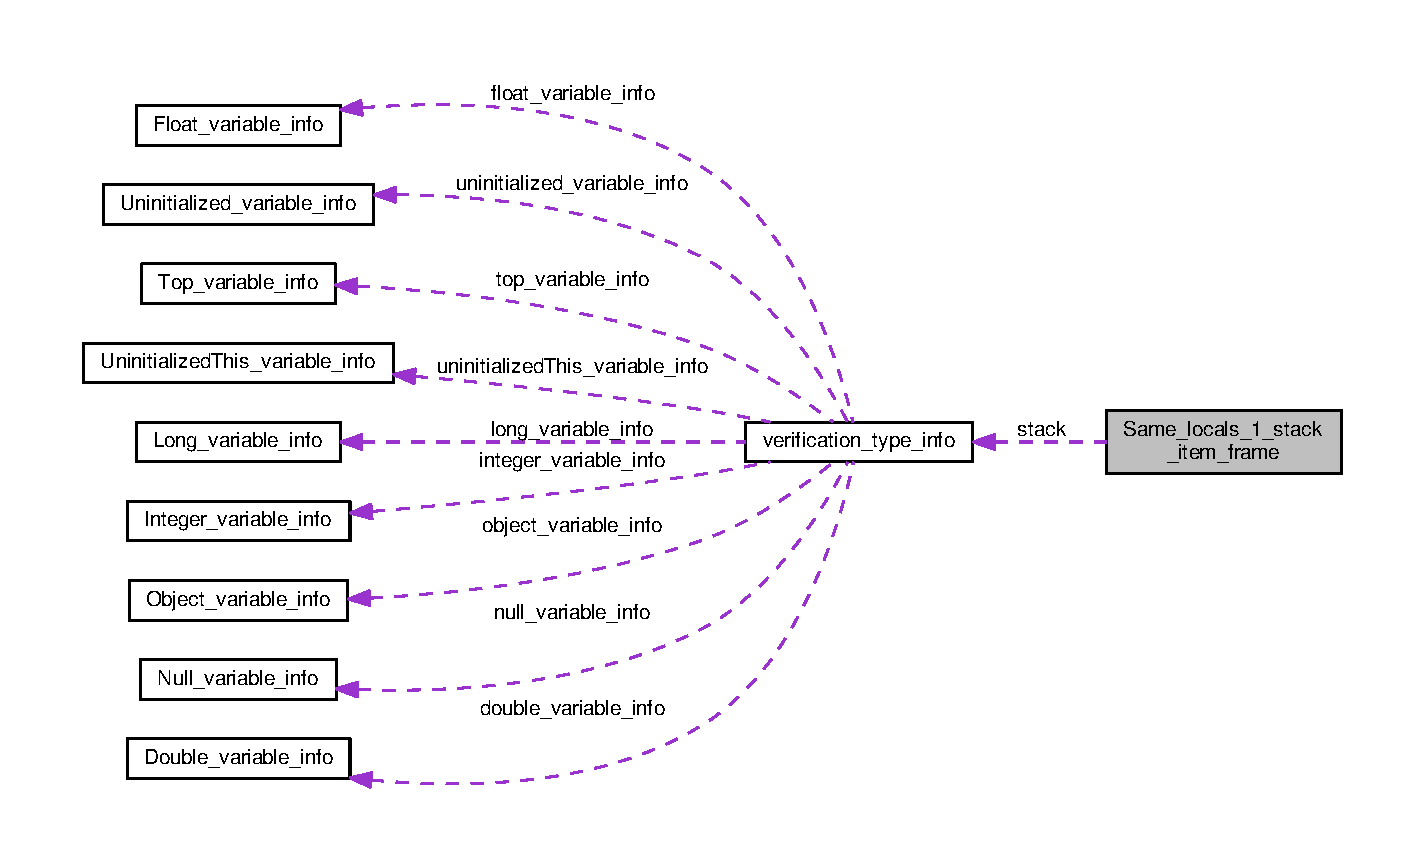
\includegraphics[width=350pt]{structSame__locals__1__stack__item__frame__coll__graph}
\end{center}
\end{figure}
\subsection*{Public Attributes}
\begin{DoxyCompactItemize}
\item 
\hyperlink{structverification__type__info}{verification\+\_\+type\+\_\+info} $\ast$ \hyperlink{structSame__locals__1__stack__item__frame_aea334c9e9f4e42aad07a6ec10a7f058a}{stack}
\end{DoxyCompactItemize}


\subsection{Member Data Documentation}
\index{Same\+\_\+locals\+\_\+1\+\_\+stack\+\_\+item\+\_\+frame@{Same\+\_\+locals\+\_\+1\+\_\+stack\+\_\+item\+\_\+frame}!stack@{stack}}
\index{stack@{stack}!Same\+\_\+locals\+\_\+1\+\_\+stack\+\_\+item\+\_\+frame@{Same\+\_\+locals\+\_\+1\+\_\+stack\+\_\+item\+\_\+frame}}
\subsubsection[{\texorpdfstring{stack}{stack}}]{\setlength{\rightskip}{0pt plus 5cm}{\bf verification\+\_\+type\+\_\+info}$\ast$ Same\+\_\+locals\+\_\+1\+\_\+stack\+\_\+item\+\_\+frame\+::stack}\hypertarget{structSame__locals__1__stack__item__frame_aea334c9e9f4e42aad07a6ec10a7f058a}{}\label{structSame__locals__1__stack__item__frame_aea334c9e9f4e42aad07a6ec10a7f058a}


The documentation for this struct was generated from the following file\+:\begin{DoxyCompactItemize}
\item 
\hyperlink{structures_8h}{structures.\+h}\end{DoxyCompactItemize}

\hypertarget{structSame__locals__1__stack__item__frame__extended}{}\section{Same\+\_\+locals\+\_\+1\+\_\+stack\+\_\+item\+\_\+frame\+\_\+extended Struct Reference}
\label{structSame__locals__1__stack__item__frame__extended}\index{Same\+\_\+locals\+\_\+1\+\_\+stack\+\_\+item\+\_\+frame\+\_\+extended@{Same\+\_\+locals\+\_\+1\+\_\+stack\+\_\+item\+\_\+frame\+\_\+extended}}


Collaboration diagram for Same\+\_\+locals\+\_\+1\+\_\+stack\+\_\+item\+\_\+frame\+\_\+extended\+:
% FIG 0
\subsection*{Public Attributes}
\begin{DoxyCompactItemize}
\item 
u2 {\bfseries offset\+\_\+delta}\hypertarget{structSame__locals__1__stack__item__frame__extended_af1fb0ce3ba68c6d6b49992b99a044235}{}\label{structSame__locals__1__stack__item__frame__extended_af1fb0ce3ba68c6d6b49992b99a044235}

\item 
\hyperlink{structverification__type__info}{verification\+\_\+type\+\_\+info} $\ast$ {\bfseries stack}\hypertarget{structSame__locals__1__stack__item__frame__extended_a7900584b7fadb413da796fbd30c1fa2b}{}\label{structSame__locals__1__stack__item__frame__extended_a7900584b7fadb413da796fbd30c1fa2b}

\end{DoxyCompactItemize}


The documentation for this struct was generated from the following file\+:\begin{DoxyCompactItemize}
\item 
structures.\+h\end{DoxyCompactItemize}

\hypertarget{structstack__map__frame}{}\section{stack\+\_\+map\+\_\+frame Struct Reference}
\label{structstack__map__frame}\index{stack\+\_\+map\+\_\+frame@{stack\+\_\+map\+\_\+frame}}


{\ttfamily \#include $<$structures.\+h$>$}



Collaboration diagram for stack\+\_\+map\+\_\+frame\+:
\nopagebreak
\begin{figure}[H]
\begin{center}
\leavevmode
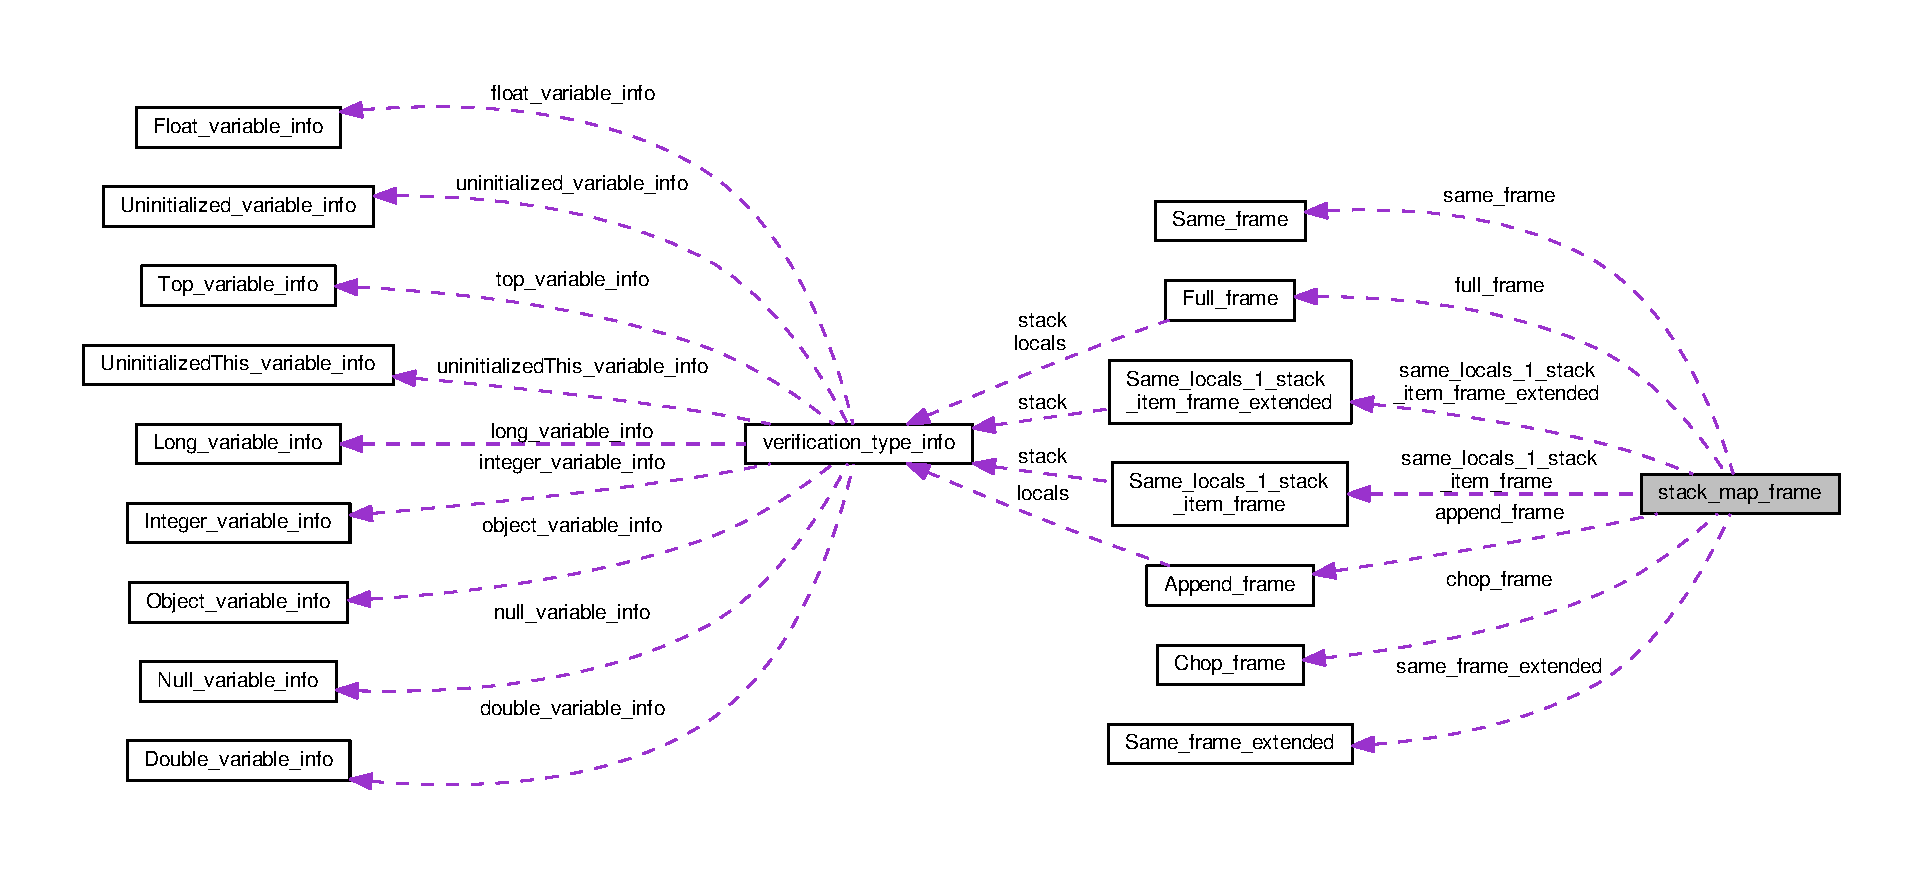
\includegraphics[width=350pt]{structstack__map__frame__coll__graph}
\end{center}
\end{figure}
\subsection*{Public Attributes}
\begin{DoxyCompactItemize}
\item 
\hyperlink{structures_8h_a64f8055b64cf2a4c299c841130c5c938}{u1} \hyperlink{structstack__map__frame_ae7d53e0f8daea6d5738a88ffb94e575c}{frame\+\_\+type}
\item 
\begin{tabbing}
xx\=xx\=xx\=xx\=xx\=xx\=xx\=xx\=xx\=\kill
union \{\\
\>\hyperlink{structSame__frame}{Same\_frame} \hyperlink{structstack__map__frame_a566369b2c76e233dc18856709be7d3dc}{same\_frame}\\
\>\hyperlink{structSame__locals__1__stack__item__frame}{Same\_locals\_1\_stack\_item\_frame} \hyperlink{structstack__map__frame_a4a73bdea158110c9c632ef657acdceed}{same\_locals\_1\_stack\_item\_frame}\\
\>\hyperlink{structSame__locals__1__stack__item__frame__extended}{Same\_locals\_1\_stack\_item\_frame\_extended} \hyperlink{structstack__map__frame_acb0262b85b6ddf629227b4e269107c4d}{same\_locals\_1\_stack\_item\_frame\_extended}\\
\>\hyperlink{structChop__frame}{Chop\_frame} \hyperlink{structstack__map__frame_a5240372d8b1af1775ee49050a515b9f2}{chop\_frame}\\
\>\hyperlink{structSame__frame__extended}{Same\_frame\_extended} \hyperlink{structstack__map__frame_a5fd4fb1c466520e7296b33ca512a844a}{same\_frame\_extended}\\
\>\hyperlink{structAppend__frame}{Append\_frame} \hyperlink{structstack__map__frame_ab412797c19922cdc0ac8fee59c59b49b}{append\_frame}\\
\>\hyperlink{structFull__frame}{Full\_frame} \hyperlink{structstack__map__frame_a6f51b3460b916cc6285c57efa37bf8e0}{full\_frame}\\
\}; \\

\end{tabbing}\end{DoxyCompactItemize}


\subsection{Member Data Documentation}
\subsubsection[{\texorpdfstring{"@23}{@23}}]{\setlength{\rightskip}{0pt plus 5cm}union \{ ... \} }\hypertarget{structstack__map__frame_a5c073aea2bad69d9058ef668105484da}{}\label{structstack__map__frame_a5c073aea2bad69d9058ef668105484da}
\index{stack\+\_\+map\+\_\+frame@{stack\+\_\+map\+\_\+frame}!append\+\_\+frame@{append\+\_\+frame}}
\index{append\+\_\+frame@{append\+\_\+frame}!stack\+\_\+map\+\_\+frame@{stack\+\_\+map\+\_\+frame}}
\subsubsection[{\texorpdfstring{append\+\_\+frame}{append_frame}}]{\setlength{\rightskip}{0pt plus 5cm}{\bf Append\+\_\+frame} stack\+\_\+map\+\_\+frame\+::append\+\_\+frame}\hypertarget{structstack__map__frame_ab412797c19922cdc0ac8fee59c59b49b}{}\label{structstack__map__frame_ab412797c19922cdc0ac8fee59c59b49b}
\index{stack\+\_\+map\+\_\+frame@{stack\+\_\+map\+\_\+frame}!chop\+\_\+frame@{chop\+\_\+frame}}
\index{chop\+\_\+frame@{chop\+\_\+frame}!stack\+\_\+map\+\_\+frame@{stack\+\_\+map\+\_\+frame}}
\subsubsection[{\texorpdfstring{chop\+\_\+frame}{chop_frame}}]{\setlength{\rightskip}{0pt plus 5cm}{\bf Chop\+\_\+frame} stack\+\_\+map\+\_\+frame\+::chop\+\_\+frame}\hypertarget{structstack__map__frame_a5240372d8b1af1775ee49050a515b9f2}{}\label{structstack__map__frame_a5240372d8b1af1775ee49050a515b9f2}
\index{stack\+\_\+map\+\_\+frame@{stack\+\_\+map\+\_\+frame}!frame\+\_\+type@{frame\+\_\+type}}
\index{frame\+\_\+type@{frame\+\_\+type}!stack\+\_\+map\+\_\+frame@{stack\+\_\+map\+\_\+frame}}
\subsubsection[{\texorpdfstring{frame\+\_\+type}{frame_type}}]{\setlength{\rightskip}{0pt plus 5cm}{\bf u1} stack\+\_\+map\+\_\+frame\+::frame\+\_\+type}\hypertarget{structstack__map__frame_ae7d53e0f8daea6d5738a88ffb94e575c}{}\label{structstack__map__frame_ae7d53e0f8daea6d5738a88ffb94e575c}
\index{stack\+\_\+map\+\_\+frame@{stack\+\_\+map\+\_\+frame}!full\+\_\+frame@{full\+\_\+frame}}
\index{full\+\_\+frame@{full\+\_\+frame}!stack\+\_\+map\+\_\+frame@{stack\+\_\+map\+\_\+frame}}
\subsubsection[{\texorpdfstring{full\+\_\+frame}{full_frame}}]{\setlength{\rightskip}{0pt plus 5cm}{\bf Full\+\_\+frame} stack\+\_\+map\+\_\+frame\+::full\+\_\+frame}\hypertarget{structstack__map__frame_a6f51b3460b916cc6285c57efa37bf8e0}{}\label{structstack__map__frame_a6f51b3460b916cc6285c57efa37bf8e0}
\index{stack\+\_\+map\+\_\+frame@{stack\+\_\+map\+\_\+frame}!same\+\_\+frame@{same\+\_\+frame}}
\index{same\+\_\+frame@{same\+\_\+frame}!stack\+\_\+map\+\_\+frame@{stack\+\_\+map\+\_\+frame}}
\subsubsection[{\texorpdfstring{same\+\_\+frame}{same_frame}}]{\setlength{\rightskip}{0pt plus 5cm}{\bf Same\+\_\+frame} stack\+\_\+map\+\_\+frame\+::same\+\_\+frame}\hypertarget{structstack__map__frame_a566369b2c76e233dc18856709be7d3dc}{}\label{structstack__map__frame_a566369b2c76e233dc18856709be7d3dc}
\index{stack\+\_\+map\+\_\+frame@{stack\+\_\+map\+\_\+frame}!same\+\_\+frame\+\_\+extended@{same\+\_\+frame\+\_\+extended}}
\index{same\+\_\+frame\+\_\+extended@{same\+\_\+frame\+\_\+extended}!stack\+\_\+map\+\_\+frame@{stack\+\_\+map\+\_\+frame}}
\subsubsection[{\texorpdfstring{same\+\_\+frame\+\_\+extended}{same_frame_extended}}]{\setlength{\rightskip}{0pt plus 5cm}{\bf Same\+\_\+frame\+\_\+extended} stack\+\_\+map\+\_\+frame\+::same\+\_\+frame\+\_\+extended}\hypertarget{structstack__map__frame_a5fd4fb1c466520e7296b33ca512a844a}{}\label{structstack__map__frame_a5fd4fb1c466520e7296b33ca512a844a}
\index{stack\+\_\+map\+\_\+frame@{stack\+\_\+map\+\_\+frame}!same\+\_\+locals\+\_\+1\+\_\+stack\+\_\+item\+\_\+frame@{same\+\_\+locals\+\_\+1\+\_\+stack\+\_\+item\+\_\+frame}}
\index{same\+\_\+locals\+\_\+1\+\_\+stack\+\_\+item\+\_\+frame@{same\+\_\+locals\+\_\+1\+\_\+stack\+\_\+item\+\_\+frame}!stack\+\_\+map\+\_\+frame@{stack\+\_\+map\+\_\+frame}}
\subsubsection[{\texorpdfstring{same\+\_\+locals\+\_\+1\+\_\+stack\+\_\+item\+\_\+frame}{same_locals_1_stack_item_frame}}]{\setlength{\rightskip}{0pt plus 5cm}{\bf Same\+\_\+locals\+\_\+1\+\_\+stack\+\_\+item\+\_\+frame} stack\+\_\+map\+\_\+frame\+::same\+\_\+locals\+\_\+1\+\_\+stack\+\_\+item\+\_\+frame}\hypertarget{structstack__map__frame_a4a73bdea158110c9c632ef657acdceed}{}\label{structstack__map__frame_a4a73bdea158110c9c632ef657acdceed}
\index{stack\+\_\+map\+\_\+frame@{stack\+\_\+map\+\_\+frame}!same\+\_\+locals\+\_\+1\+\_\+stack\+\_\+item\+\_\+frame\+\_\+extended@{same\+\_\+locals\+\_\+1\+\_\+stack\+\_\+item\+\_\+frame\+\_\+extended}}
\index{same\+\_\+locals\+\_\+1\+\_\+stack\+\_\+item\+\_\+frame\+\_\+extended@{same\+\_\+locals\+\_\+1\+\_\+stack\+\_\+item\+\_\+frame\+\_\+extended}!stack\+\_\+map\+\_\+frame@{stack\+\_\+map\+\_\+frame}}
\subsubsection[{\texorpdfstring{same\+\_\+locals\+\_\+1\+\_\+stack\+\_\+item\+\_\+frame\+\_\+extended}{same_locals_1_stack_item_frame_extended}}]{\setlength{\rightskip}{0pt plus 5cm}{\bf Same\+\_\+locals\+\_\+1\+\_\+stack\+\_\+item\+\_\+frame\+\_\+extended} stack\+\_\+map\+\_\+frame\+::same\+\_\+locals\+\_\+1\+\_\+stack\+\_\+item\+\_\+frame\+\_\+extended}\hypertarget{structstack__map__frame_acb0262b85b6ddf629227b4e269107c4d}{}\label{structstack__map__frame_acb0262b85b6ddf629227b4e269107c4d}


The documentation for this struct was generated from the following file\+:\begin{DoxyCompactItemize}
\item 
\hyperlink{structures_8h}{structures.\+h}\end{DoxyCompactItemize}

\hypertarget{structStackFrame}{}\section{Stack\+Frame Struct Reference}
\label{structStackFrame}\index{Stack\+Frame@{Stack\+Frame}}


{\ttfamily \#include $<$stack\+\_\+frame.\+h$>$}



Collaboration diagram for Stack\+Frame\+:
% FIG 0
\subsection*{Public Attributes}
\begin{DoxyCompactItemize}
\item 
\hyperlink{structFrame}{Frame} $\ast$ \hyperlink{structStackFrame_a344a354f24d9c4b6c805cd0a029100b9}{f}
\item 
struct \hyperlink{structStackFrame}{Stack\+Frame} $\ast$ \hyperlink{structStackFrame_aae670075795a607599420fd8b5181292}{pointer}
\item 
struct \hyperlink{structStackFrame}{Stack\+Frame} $\ast$ \hyperlink{structStackFrame_a9f0df83101cacbe812d0d4b3c6e08494}{top}
\end{DoxyCompactItemize}


\subsection{Member Data Documentation}
\index{Stack\+Frame@{Stack\+Frame}!f@{f}}
\index{f@{f}!Stack\+Frame@{Stack\+Frame}}
\subsubsection[{\texorpdfstring{f}{f}}]{\setlength{\rightskip}{0pt plus 5cm}{\bf Frame}$\ast$ Stack\+Frame\+::f}\hypertarget{structStackFrame_a344a354f24d9c4b6c805cd0a029100b9}{}\label{structStackFrame_a344a354f24d9c4b6c805cd0a029100b9}
\index{Stack\+Frame@{Stack\+Frame}!pointer@{pointer}}
\index{pointer@{pointer}!Stack\+Frame@{Stack\+Frame}}
\subsubsection[{\texorpdfstring{pointer}{pointer}}]{\setlength{\rightskip}{0pt plus 5cm}struct {\bf Stack\+Frame}$\ast$ Stack\+Frame\+::pointer}\hypertarget{structStackFrame_aae670075795a607599420fd8b5181292}{}\label{structStackFrame_aae670075795a607599420fd8b5181292}
\index{Stack\+Frame@{Stack\+Frame}!top@{top}}
\index{top@{top}!Stack\+Frame@{Stack\+Frame}}
\subsubsection[{\texorpdfstring{top}{top}}]{\setlength{\rightskip}{0pt plus 5cm}struct {\bf Stack\+Frame}$\ast$ Stack\+Frame\+::top}\hypertarget{structStackFrame_a9f0df83101cacbe812d0d4b3c6e08494}{}\label{structStackFrame_a9f0df83101cacbe812d0d4b3c6e08494}


The documentation for this struct was generated from the following file\+:\begin{DoxyCompactItemize}
\item 
\hyperlink{stack__frame_8h}{stack\+\_\+frame.\+h}\end{DoxyCompactItemize}

\hypertarget{structStackOperand}{}\section{Stack\+Operand Struct Reference}
\label{structStackOperand}\index{Stack\+Operand@{Stack\+Operand}}


Estrutura que representa um operando da pilha.  




{\ttfamily \#include $<$stack\+\_\+operands.\+h$>$}



Collaboration diagram for Stack\+Operand\+:
% FIG 0
\subsection*{Public Attributes}
\begin{DoxyCompactItemize}
\item 
\hyperlink{structLocalVariable}{Local\+Variable} $\ast$ \hyperlink{structStackOperand_ac2430d118d01240603507706e8a8adff}{f}
\item 
struct \hyperlink{structStackOperand}{Stack\+Operand} $\ast$ \hyperlink{structStackOperand_af4ad4c3c4e49be261c61b3856bc02b9f}{pointer}
\item 
struct \hyperlink{structStackOperand}{Stack\+Operand} $\ast$ \hyperlink{structStackOperand_a11a33c73ab08f65a14fb53af2308d052}{top}
\end{DoxyCompactItemize}


\subsection{Detailed Description}
Estrutura que representa um operando da pilha. 

Struct que implementa a pilha de operandos.

Possui um ponteiro para uma \hyperlink{structLocalVariable}{Local\+Variable} e um pointeiro para uma pilha de operandos. 

\subsection{Member Data Documentation}
\index{Stack\+Operand@{Stack\+Operand}!f@{f}}
\index{f@{f}!Stack\+Operand@{Stack\+Operand}}
\subsubsection[{\texorpdfstring{f}{f}}]{\setlength{\rightskip}{0pt plus 5cm}{\bf Local\+Variable}$\ast$ Stack\+Operand\+::f}\hypertarget{structStackOperand_ac2430d118d01240603507706e8a8adff}{}\label{structStackOperand_ac2430d118d01240603507706e8a8adff}
\index{Stack\+Operand@{Stack\+Operand}!pointer@{pointer}}
\index{pointer@{pointer}!Stack\+Operand@{Stack\+Operand}}
\subsubsection[{\texorpdfstring{pointer}{pointer}}]{\setlength{\rightskip}{0pt plus 5cm}struct {\bf Stack\+Operand}$\ast$ Stack\+Operand\+::pointer}\hypertarget{structStackOperand_af4ad4c3c4e49be261c61b3856bc02b9f}{}\label{structStackOperand_af4ad4c3c4e49be261c61b3856bc02b9f}
\index{Stack\+Operand@{Stack\+Operand}!top@{top}}
\index{top@{top}!Stack\+Operand@{Stack\+Operand}}
\subsubsection[{\texorpdfstring{top}{top}}]{\setlength{\rightskip}{0pt plus 5cm}struct {\bf Stack\+Operand}$\ast$ Stack\+Operand\+::top}\hypertarget{structStackOperand_a11a33c73ab08f65a14fb53af2308d052}{}\label{structStackOperand_a11a33c73ab08f65a14fb53af2308d052}


The documentation for this struct was generated from the following file\+:\begin{DoxyCompactItemize}
\item 
\hyperlink{stack__operands_8h}{stack\+\_\+operands.\+h}\end{DoxyCompactItemize}

\hypertarget{structTop__variable__info}{}\section{Top\+\_\+variable\+\_\+info Struct Reference}
\label{structTop__variable__info}\index{Top\+\_\+variable\+\_\+info@{Top\+\_\+variable\+\_\+info}}


{\ttfamily \#include $<$structures.\+h$>$}



The documentation for this struct was generated from the following file\+:\begin{DoxyCompactItemize}
\item 
\hyperlink{structures_8h}{structures.\+h}\end{DoxyCompactItemize}

\hypertarget{structTypeArray}{}\section{Type\+Array Struct Reference}
\label{structTypeArray}\index{Type\+Array@{Type\+Array}}


{\ttfamily \#include $<$structures.\+h$>$}

\subsection*{Public Attributes}
\begin{DoxyCompactItemize}
\item 
void $\ast$ \hyperlink{structTypeArray_a6126c1f56950b1821af98aa19d4c5cdc}{array}
\item 
\hyperlink{structures_8h_a55ef8d87fd202b8417704c089899c5b9}{u2} \hyperlink{structTypeArray_a51c37b7d51078be5f6f6dc83c58fdb22}{size}
\end{DoxyCompactItemize}


\subsection{Member Data Documentation}
\index{Type\+Array@{Type\+Array}!array@{array}}
\index{array@{array}!Type\+Array@{Type\+Array}}
\subsubsection[{\texorpdfstring{array}{array}}]{\setlength{\rightskip}{0pt plus 5cm}void$\ast$ Type\+Array\+::array}\hypertarget{structTypeArray_a6126c1f56950b1821af98aa19d4c5cdc}{}\label{structTypeArray_a6126c1f56950b1821af98aa19d4c5cdc}
\index{Type\+Array@{Type\+Array}!size@{size}}
\index{size@{size}!Type\+Array@{Type\+Array}}
\subsubsection[{\texorpdfstring{size}{size}}]{\setlength{\rightskip}{0pt plus 5cm}{\bf u2} Type\+Array\+::size}\hypertarget{structTypeArray_a51c37b7d51078be5f6f6dc83c58fdb22}{}\label{structTypeArray_a51c37b7d51078be5f6f6dc83c58fdb22}


The documentation for this struct was generated from the following file\+:\begin{DoxyCompactItemize}
\item 
\hyperlink{structures_8h}{structures.\+h}\end{DoxyCompactItemize}

\hypertarget{structUninitialized__variable__info}{}\section{Uninitialized\+\_\+variable\+\_\+info Struct Reference}
\label{structUninitialized__variable__info}\index{Uninitialized\+\_\+variable\+\_\+info@{Uninitialized\+\_\+variable\+\_\+info}}


{\ttfamily \#include $<$structures.\+h$>$}

\subsection*{Public Attributes}
\begin{DoxyCompactItemize}
\item 
\hyperlink{structures_8h_a55ef8d87fd202b8417704c089899c5b9}{u2} \hyperlink{structUninitialized__variable__info_aa80d6f40ad156843843eedf9b03f9add}{offset}
\end{DoxyCompactItemize}


\subsection{Member Data Documentation}
\index{Uninitialized\+\_\+variable\+\_\+info@{Uninitialized\+\_\+variable\+\_\+info}!offset@{offset}}
\index{offset@{offset}!Uninitialized\+\_\+variable\+\_\+info@{Uninitialized\+\_\+variable\+\_\+info}}
\subsubsection[{\texorpdfstring{offset}{offset}}]{\setlength{\rightskip}{0pt plus 5cm}{\bf u2} Uninitialized\+\_\+variable\+\_\+info\+::offset}\hypertarget{structUninitialized__variable__info_aa80d6f40ad156843843eedf9b03f9add}{}\label{structUninitialized__variable__info_aa80d6f40ad156843843eedf9b03f9add}


The documentation for this struct was generated from the following file\+:\begin{DoxyCompactItemize}
\item 
\hyperlink{structures_8h}{structures.\+h}\end{DoxyCompactItemize}

\hypertarget{structUninitializedThis__variable__info}{}\section{Uninitialized\+This\+\_\+variable\+\_\+info Struct Reference}
\label{structUninitializedThis__variable__info}\index{Uninitialized\+This\+\_\+variable\+\_\+info@{Uninitialized\+This\+\_\+variable\+\_\+info}}


{\ttfamily \#include $<$structures.\+h$>$}



The documentation for this struct was generated from the following file\+:\begin{DoxyCompactItemize}
\item 
\hyperlink{structures_8h}{structures.\+h}\end{DoxyCompactItemize}

\hypertarget{structverification__type__info}{}\section{verification\+\_\+type\+\_\+info Struct Reference}
\label{structverification__type__info}\index{verification\+\_\+type\+\_\+info@{verification\+\_\+type\+\_\+info}}


{\ttfamily \#include $<$structures.\+h$>$}



Collaboration diagram for verification\+\_\+type\+\_\+info\+:
% FIG 0
\subsection*{Public Attributes}
\begin{DoxyCompactItemize}
\item 
\hyperlink{structures_8h_a64f8055b64cf2a4c299c841130c5c938}{u1} \hyperlink{structverification__type__info_aeb9c72b398b4d3ce0863a916f973b05c}{tag}
\item 
\begin{tabbing}
xx\=xx\=xx\=xx\=xx\=xx\=xx\=xx\=xx\=\kill
union \{\\
\>\hyperlink{structTop__variable__info}{Top\_variable\_info} \hyperlink{structverification__type__info_aa9c08dabdcc9eb9cd6887ffc1b7acdb0}{top\_variable\_info}\\
\>\hyperlink{structInteger__variable__info}{Integer\_variable\_info} \hyperlink{structverification__type__info_aa0eb61689487e7851038e8e0ba37a6b6}{integer\_variable\_info}\\
\>\hyperlink{structFloat__variable__info}{Float\_variable\_info} \hyperlink{structverification__type__info_a73db385fdde1fdd46b6ff6386bf28320}{float\_variable\_info}\\
\>\hyperlink{structLong__variable__info}{Long\_variable\_info} \hyperlink{structverification__type__info_a2d890836853a27c0f4bff1b135b3d844}{long\_variable\_info}\\
\>\hyperlink{structDouble__variable__info}{Double\_variable\_info} \hyperlink{structverification__type__info_ac01c6db2b8dd5bfe47a98a2ec2528448}{double\_variable\_info}\\
\>\hyperlink{structNull__variable__info}{Null\_variable\_info} \hyperlink{structverification__type__info_a1f4205281e4346364160c3929783befc}{null\_variable\_info}\\
\>\hyperlink{structUninitializedThis__variable__info}{UninitializedThis\_variable\_info} \hyperlink{structverification__type__info_a40830fd30b55a46a26d9c209bba7b3a8}{uninitializedThis\_variable\_info}\\
\>\hyperlink{structObject__variable__info}{Object\_variable\_info} \hyperlink{structverification__type__info_a7efcdeee31cb5c174267bf13a7386f31}{object\_variable\_info}\\
\>\hyperlink{structUninitialized__variable__info}{Uninitialized\_variable\_info} \hyperlink{structverification__type__info_a036f3ae811e853852803f816c0d69933}{uninitialized\_variable\_info}\\
\}; \\

\end{tabbing}\end{DoxyCompactItemize}


\subsection{Member Data Documentation}
\subsubsection[{\texorpdfstring{"@21}{@21}}]{\setlength{\rightskip}{0pt plus 5cm}union \{ ... \} }\hypertarget{structverification__type__info_a742e5022806c973ace237c359897885c}{}\label{structverification__type__info_a742e5022806c973ace237c359897885c}
\index{verification\+\_\+type\+\_\+info@{verification\+\_\+type\+\_\+info}!double\+\_\+variable\+\_\+info@{double\+\_\+variable\+\_\+info}}
\index{double\+\_\+variable\+\_\+info@{double\+\_\+variable\+\_\+info}!verification\+\_\+type\+\_\+info@{verification\+\_\+type\+\_\+info}}
\subsubsection[{\texorpdfstring{double\+\_\+variable\+\_\+info}{double_variable_info}}]{\setlength{\rightskip}{0pt plus 5cm}{\bf Double\+\_\+variable\+\_\+info} verification\+\_\+type\+\_\+info\+::double\+\_\+variable\+\_\+info}\hypertarget{structverification__type__info_ac01c6db2b8dd5bfe47a98a2ec2528448}{}\label{structverification__type__info_ac01c6db2b8dd5bfe47a98a2ec2528448}
\index{verification\+\_\+type\+\_\+info@{verification\+\_\+type\+\_\+info}!float\+\_\+variable\+\_\+info@{float\+\_\+variable\+\_\+info}}
\index{float\+\_\+variable\+\_\+info@{float\+\_\+variable\+\_\+info}!verification\+\_\+type\+\_\+info@{verification\+\_\+type\+\_\+info}}
\subsubsection[{\texorpdfstring{float\+\_\+variable\+\_\+info}{float_variable_info}}]{\setlength{\rightskip}{0pt plus 5cm}{\bf Float\+\_\+variable\+\_\+info} verification\+\_\+type\+\_\+info\+::float\+\_\+variable\+\_\+info}\hypertarget{structverification__type__info_a73db385fdde1fdd46b6ff6386bf28320}{}\label{structverification__type__info_a73db385fdde1fdd46b6ff6386bf28320}
\index{verification\+\_\+type\+\_\+info@{verification\+\_\+type\+\_\+info}!integer\+\_\+variable\+\_\+info@{integer\+\_\+variable\+\_\+info}}
\index{integer\+\_\+variable\+\_\+info@{integer\+\_\+variable\+\_\+info}!verification\+\_\+type\+\_\+info@{verification\+\_\+type\+\_\+info}}
\subsubsection[{\texorpdfstring{integer\+\_\+variable\+\_\+info}{integer_variable_info}}]{\setlength{\rightskip}{0pt plus 5cm}{\bf Integer\+\_\+variable\+\_\+info} verification\+\_\+type\+\_\+info\+::integer\+\_\+variable\+\_\+info}\hypertarget{structverification__type__info_aa0eb61689487e7851038e8e0ba37a6b6}{}\label{structverification__type__info_aa0eb61689487e7851038e8e0ba37a6b6}
\index{verification\+\_\+type\+\_\+info@{verification\+\_\+type\+\_\+info}!long\+\_\+variable\+\_\+info@{long\+\_\+variable\+\_\+info}}
\index{long\+\_\+variable\+\_\+info@{long\+\_\+variable\+\_\+info}!verification\+\_\+type\+\_\+info@{verification\+\_\+type\+\_\+info}}
\subsubsection[{\texorpdfstring{long\+\_\+variable\+\_\+info}{long_variable_info}}]{\setlength{\rightskip}{0pt plus 5cm}{\bf Long\+\_\+variable\+\_\+info} verification\+\_\+type\+\_\+info\+::long\+\_\+variable\+\_\+info}\hypertarget{structverification__type__info_a2d890836853a27c0f4bff1b135b3d844}{}\label{structverification__type__info_a2d890836853a27c0f4bff1b135b3d844}
\index{verification\+\_\+type\+\_\+info@{verification\+\_\+type\+\_\+info}!null\+\_\+variable\+\_\+info@{null\+\_\+variable\+\_\+info}}
\index{null\+\_\+variable\+\_\+info@{null\+\_\+variable\+\_\+info}!verification\+\_\+type\+\_\+info@{verification\+\_\+type\+\_\+info}}
\subsubsection[{\texorpdfstring{null\+\_\+variable\+\_\+info}{null_variable_info}}]{\setlength{\rightskip}{0pt plus 5cm}{\bf Null\+\_\+variable\+\_\+info} verification\+\_\+type\+\_\+info\+::null\+\_\+variable\+\_\+info}\hypertarget{structverification__type__info_a1f4205281e4346364160c3929783befc}{}\label{structverification__type__info_a1f4205281e4346364160c3929783befc}
\index{verification\+\_\+type\+\_\+info@{verification\+\_\+type\+\_\+info}!object\+\_\+variable\+\_\+info@{object\+\_\+variable\+\_\+info}}
\index{object\+\_\+variable\+\_\+info@{object\+\_\+variable\+\_\+info}!verification\+\_\+type\+\_\+info@{verification\+\_\+type\+\_\+info}}
\subsubsection[{\texorpdfstring{object\+\_\+variable\+\_\+info}{object_variable_info}}]{\setlength{\rightskip}{0pt plus 5cm}{\bf Object\+\_\+variable\+\_\+info} verification\+\_\+type\+\_\+info\+::object\+\_\+variable\+\_\+info}\hypertarget{structverification__type__info_a7efcdeee31cb5c174267bf13a7386f31}{}\label{structverification__type__info_a7efcdeee31cb5c174267bf13a7386f31}
\index{verification\+\_\+type\+\_\+info@{verification\+\_\+type\+\_\+info}!tag@{tag}}
\index{tag@{tag}!verification\+\_\+type\+\_\+info@{verification\+\_\+type\+\_\+info}}
\subsubsection[{\texorpdfstring{tag}{tag}}]{\setlength{\rightskip}{0pt plus 5cm}{\bf u1} verification\+\_\+type\+\_\+info\+::tag}\hypertarget{structverification__type__info_aeb9c72b398b4d3ce0863a916f973b05c}{}\label{structverification__type__info_aeb9c72b398b4d3ce0863a916f973b05c}
\index{verification\+\_\+type\+\_\+info@{verification\+\_\+type\+\_\+info}!top\+\_\+variable\+\_\+info@{top\+\_\+variable\+\_\+info}}
\index{top\+\_\+variable\+\_\+info@{top\+\_\+variable\+\_\+info}!verification\+\_\+type\+\_\+info@{verification\+\_\+type\+\_\+info}}
\subsubsection[{\texorpdfstring{top\+\_\+variable\+\_\+info}{top_variable_info}}]{\setlength{\rightskip}{0pt plus 5cm}{\bf Top\+\_\+variable\+\_\+info} verification\+\_\+type\+\_\+info\+::top\+\_\+variable\+\_\+info}\hypertarget{structverification__type__info_aa9c08dabdcc9eb9cd6887ffc1b7acdb0}{}\label{structverification__type__info_aa9c08dabdcc9eb9cd6887ffc1b7acdb0}
\index{verification\+\_\+type\+\_\+info@{verification\+\_\+type\+\_\+info}!uninitialized\+\_\+variable\+\_\+info@{uninitialized\+\_\+variable\+\_\+info}}
\index{uninitialized\+\_\+variable\+\_\+info@{uninitialized\+\_\+variable\+\_\+info}!verification\+\_\+type\+\_\+info@{verification\+\_\+type\+\_\+info}}
\subsubsection[{\texorpdfstring{uninitialized\+\_\+variable\+\_\+info}{uninitialized_variable_info}}]{\setlength{\rightskip}{0pt plus 5cm}{\bf Uninitialized\+\_\+variable\+\_\+info} verification\+\_\+type\+\_\+info\+::uninitialized\+\_\+variable\+\_\+info}\hypertarget{structverification__type__info_a036f3ae811e853852803f816c0d69933}{}\label{structverification__type__info_a036f3ae811e853852803f816c0d69933}
\index{verification\+\_\+type\+\_\+info@{verification\+\_\+type\+\_\+info}!uninitialized\+This\+\_\+variable\+\_\+info@{uninitialized\+This\+\_\+variable\+\_\+info}}
\index{uninitialized\+This\+\_\+variable\+\_\+info@{uninitialized\+This\+\_\+variable\+\_\+info}!verification\+\_\+type\+\_\+info@{verification\+\_\+type\+\_\+info}}
\subsubsection[{\texorpdfstring{uninitialized\+This\+\_\+variable\+\_\+info}{uninitializedThis_variable_info}}]{\setlength{\rightskip}{0pt plus 5cm}{\bf Uninitialized\+This\+\_\+variable\+\_\+info} verification\+\_\+type\+\_\+info\+::uninitialized\+This\+\_\+variable\+\_\+info}\hypertarget{structverification__type__info_a40830fd30b55a46a26d9c209bba7b3a8}{}\label{structverification__type__info_a40830fd30b55a46a26d9c209bba7b3a8}


The documentation for this struct was generated from the following file\+:\begin{DoxyCompactItemize}
\item 
\hyperlink{structures_8h}{structures.\+h}\end{DoxyCompactItemize}

%--- End generated contents ---

% Index
\backmatter
\newpage
\phantomsection
\clearemptydoublepage
\addcontentsline{toc}{chapter}{Index}
\printindex

\end{document}
